%\documentclass[iop]{emulateapj}
\documentclass[preprint]{aastex}
%\documentclass[12pt, onecolumn]{emulateapj}
%\documentstyle[aas2pp4,natbib209]{article}

\usepackage{tikz}
\usepackage{natbib}
\usepackage{amsmath}

\usetikzlibrary{shapes.geometric, arrows}
\usetikzlibrary{fit}

\tikzstyle{hyper} = [circle, text centered, draw=black]%, fill=blue!30]
\tikzstyle{param} = [circle, text centered, draw=black]%, fill=green!30]
\tikzstyle{data} = [circle, text centered, draw=black, line width=2pt]%, 
fill=red!30]
%\tikzstyle{hyper} = [trapezium, trapezium left angle=70, trapezium right 
angle=110, minimum width=1cm, minimum height=0.5cm, text centered, draw=black, 
fill=green!30]
%\tikzstyle{param} = [rectangle, minimum width=1cm, minimum height=0.5cm, text 
centered, draw=black, fill=green!30]
%\tikzstyle{data} = [diamond, minimum width=1cm, minimum height=1cm, text 
centered, draw=black, fill=red!30]
%\tikzstyle{eqn} = [rectangle, minimum width=1cm, minimum height=0.5cm, text 
centered, draw=black]%, fill=green!30]
%\tikzstyle{latent} = [diamond, minimum width=1cm, minimum height=0.5cm, text 
centered, draw=black]%, fill=green!30]
\tikzstyle{arrow} = [thick,->,>=stealth]

\newcommand{\myemail}{aimalz@nyu.edu}
\newcommand{\textul}{\underline}

\shorttitle{A Probabilistic Approach to the Redshift Distribution Function}
\shortauthors{Malz and Hogg}

\begin{document}

\title{A Fully Probabilistic Approach to the Redshift Distribution Function}

\author{A.I. Malz\altaffilmark{1}}
\email{aimalz@nyu.edu}

\author{D.W. Hogg\altaffilmark{1}}
\email{david.hogg@nyu.edu}

\altaffiltext{1}{New York University Center for Cosmology and Particle Physics}

\begin{abstract}
Photometric redshift probability distribution functions are rapidly replacing 
redshift point estimates as data products of photometric galaxy surveys.  
Though there is not yet agreement on the best way to derive such data products, 
they are most commonly stacked to obtain an estimate of the redshift 
distribution function $N(z)$ necessary for weak gravitational lensing 
calculations and reduced to point estimates in calculations of more complicated 
statistics.  This work challenges that paradigm and proposes a mathematically 
consistent technique motivated by fundamental probability theory in which a 
probabilistic graphical model elucidates the relation of interim photometric 
redshift posteriors to a full posterior distribution over relevant physical 
parameters, sampled by Monte Carlo-Markov Chain procedures.  The approach is 
applied to the one-point statistic of the redshift distribution function $N(z)$ 
and validated on synthetic data.  It is demonstrated that this method improves 
accuracy compared to popular alternatives such as stacking and conversion of 
photometric redshift probability distributions to point estimates of redshift.
\end{abstract}

\keywords{photo-z}

\clearpage
\section{Introduction}
\label{sec:intro}

The era of precision cosmology, heralded by weak gravitational lensing 
tomography and baryon acoustic oscillation peak measurements, has been enabled 
by photometric estimation of redshifts previously accessible only by time- and 
resource-intensive spectroscopic confirmation.  However, photometric redshifts 
(photo-zs) are susceptible to a number of sources of error, particularly their 
inherent noisiness due to the coarseness of photometric filters, errors in 
which galaxies of one type at one redshift are mistaken for galaxies of another 
type at a different redshift, and systematics introduced by observational 
techniques and data reduction processes.  In addition to these limitations in 
accuracy, there is also the matter of precision; photo-zs are often reported 
with error bars derived without inclusion of all systematic errors, including 
the different selection effects between the magnitude-spaces of galaxies for 
which photo-zs are desired and galaxies with spectroscopically confirmed 
redshifts used to calibrate photo-z estimators.

Since their conception \citep{Baum1962}, much effort has been dedicated to 
improving photo-zs, though they are still most commonly obtained by a maximum 
likelihood estimator (MLE) based on libraries of galaxy spectral energy 
distribution (SED) templates with conservative approaches to error estimation.  
Recent work has focused on identifying and removing catastrophic outliers when 
using photo-zs for inference.  \citep{Gorecki2014}  Sophisticated Bayesian 
techniques and cutting-edge machine learning methods have been employed to 
improve precision \citep{Carliles2010} and accuracy \citep{Sadeh2015}. 

An alternative to point estimates of photo-zs is redshift probability 
distribution function estimation, in which rather than an MLE point estimate, 
the full posterior probability (or likelihood) function of the redshift of a 
galaxy is reported.  \citep{Koo1999}  This option is favorable because it 
contains more potentially useful information than a point estimate while 
addressing the issues with precision, accuracy, and systematics.  However, 
photo-z probability distribution functions are not without their own 
weaknesses, the foremost of which are the computation time and storage space 
necessary to calculate and record them for large galaxy surveys 
\citep{CarrascoKind2014} and the method used to derive them.

Many techniques to obtain photo-z probability distributions have been proposed 
and tested in the literature, but no one method has yet been generally agreed 
upon.  An extension of the Bayesian photometric redshift (BPZ) method of 
\citet{Benitez2000} that produces posterior probability distributions (as 
opposed to a selection of local maxima) from an SED template library has been 
employed.  \citep{Hildebrandt2012, Kelly2014, Lopez-Sanjuan2015}  Photo-z 
posterior probability distributions have also been obtained by a variety of 
trustworthy data-driven approaches in the literature: $k$-nearest neighbor 
algorithms with \citep{Ball2008} and without \citep{Sheldon2012} inclusion of 
photometric measurement errors, neural networks \citep{Bonnett2015a}, 
self-organizing maps \citep{CarrascoKind2014a}, and prediction tree and random 
forest classification techniques \citep{Carliles2010, CarrascoKind2013}.  (The 
approaches of fitting to a training set and fitting to a template library are 
related by \citet{Budavari2009}.)  Some current work aims to vet photo-z 
probability distribution generation methods \citep{Wittman2016}, but much 
remains to be done.

Photo-z probability distributions have been produced by completed surveys 
\citep{Hildebrandt2012, Sheldon2012} and will be produced by upcoming surveys 
\citep{LSSTScienceCollaboration2009, CarrascoKind2014a, Masters2015a}.  Though 
their potential to improve estimates of physical parameters is tremendous, 
photo-z posterior probability distributions have been applied only to a limited 
extent.  They have been used to form selection criteria of samples from galaxy 
surveys for the purpose of calculating physical parameters but have not been 
propagated through the calculations themselves.  
\citep{VanBreukelen2009,Viironen2015}  Probability cuts on Bayesian quantities 
are not uncommon \citep{Leung2015, DiPompeo2015a}, but that procedure does not 
fully take advantage of all information contained in a probability distribution 
for parameter inference.  However, no implementation of inference with photo-z 
posterior distributions has been presented with a mathematically consistent 
methodology.  The goal of this paper is to clearly present and validate a 
technique for the use of photo-z posterior distributions in inference.  For 
simplicity, we consider only one-point statistics relevant to cosmology, though 
future work will extend this methodology to higher-order statistics.

The redshift distribution function $N(z)$ serves as an ideal statistic upon 
which to demonstrate such an approach, in large part because it has been the 
subject of inference using photo-z probability distributions before.  
\citep{Sheldon2012, Hildebrandt2012, Kelly2014, Benjamin2013, Bonnett2015a, 
Viironen2015, Asorey2016}  $N(z)$ for observed galaxies can be used to validate 
survey selection functions used in generation of realistic mock catalogs used 
for many purposes.  \citep{Norberg2002}  The redshift density function $n(z)$, 
derived from $N(z)$, is also necessary for calculations of two-point 
correlation functions of weak lensing shear and counting statistics that are 
directly used to probe cosmological parameters.  \citep{Masters2015}  This 
paper will not develop a method for fully integrating photo-z probability 
distributions into calculations of two-point statistics of redshift, though 
some work has already been dedicated to that cause.  \citep{Myers2009}

\textbf{Is this sufficiently complete?  Am I missing some really important 
references?  I am worried this introduction isn't long enough.}

Sec. \ref{sec:meth} will derive the framework for exploring the full posterior 
of distribution for $N(z)$ using photo-z probability distribution functions.  
Sec. \ref{sec:exp} will describe how the model given in Sec. \ref{sec:meth} is 
implemented.  Sec. \ref{sec:valid} will discuss the results of applying the 
fully probabilistic approach to mock and real datasets.

\clearpage
\section{Method}
\label{sec:meth}

\textbf{I'm quite confident in this section as a whole.  Let me know where that 
confidence is inappropriate.}

It is best to begin with a general description of the problem at hand.  Let us 
consider a survey of $J$ galaxies $j$, each with photometric data 
$\vec{d}_{j}$; thus the entire survey over some solid angle $\Omega$ produces 
the ensemble of photometric magnitudes (or colors) and their associated 
observational errors $\{\vec{d}_{j}\}_{J}$.  Each galaxy $j$ has a redshift 
$z_{j}$ that we would like to learn; redshift is a parameter in this case.  The 
distribution of the ensemble of redshifts $\{z_{j}\}_{J}$ may be described by 
the hyperparameters defining the redshift distribution function $N(z)$ that we 
would like to quantify.  This situation may be considered to be a probabilistic 
generative model, illustrated by the directed acyclic graph of Fig. 
\ref{fig:flow}.  

\begin{figure}
\vspace{0.5cm}
\begin{center}
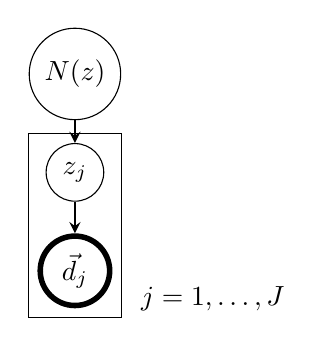
\begin{tikzpicture}[node distance=1cm]

\node (nz) [hyper] {$N(z)$};
\node (z) [param, below of=nz,yshift=-0.25cm] {$z_{j}$};
\node (mags) [data, below of=z,yshift=-0.25cm] {$\vec{d}_{j}$};
\node (survey) [draw=black,fit={(mags.west)(z.north)(mags.south)(mags.east)}] 
{};
\node [xshift=1.75cm,yshift=0.25cm] at (survey.south) {$j=1,\dots,J$};

\draw [arrow] (nz) -- (z);
\draw [arrow] (z) -- (mags);

\end{tikzpicture}
\caption{This directed acyclic graph illustrates a hierarchical model.}
\label{fig:flow}
\end{center}
\end{figure}

The redshift distribution function $N(z)$ shown in Eq. \ref{eq:distribution} 
gives the number of galaxies per unit redshift, effectively defining the 
evolution in the number of galaxies.  \citep{Menard2013}  In the following 
sections, we will present and compare methods for calculating $N(z)$ from 
photometric redshift probability distribution functions.  Sec. \ref{sec:prob} 
contains the mathematical derivation of a probabilistic model for $N(z)$ 
dependent on photo-z probability distribution functions, and Sec. 
\ref{sec:sheldon} contrasts the probabilistic model with alternative methods.

\begin{eqnarray}
\label{eq:distribution}
N(z) &=& \frac{dN}{dz}
\end{eqnarray}

\clearpage
\subsection{Probabilistic Model}
\label{sec:prob}

We begin by parametrizing $N(z)$ in terms of $\vec{\theta}$, comprising some 
set of hyperparameters that define the form $N(z)$ may take in whatever basis 
we choose.  At this point, these hyperparameters are quite general and may 
represent coefficients in a high-order polynomial as a function of redshift, a 
set of means and variances defining Gaussians that sum to the desired 
distribution, a set of histogram heights that describe a binned version of the 
redshift distribution function, etc.  We define a function 
$f_{\vec{\theta}}(z)=N(z)$ that transforms these hyperparameters into the 
redshift distribution function $N(z)$.

In this paper, we shall work exclusively with log-probabilities.  What we wish 
to estimate is the full posterior probability distribution (hereafter the full 
posterior) of the hyperparameters $\vec{\theta}$ given the data 
$\{\vec{d}_{j}\}_{J}$.  By Bayes' Rule, the full posterior 
$\ln[p(\vec{\theta}|\{\vec{d}_{j}\}_{J})]$ may be expressed in terms of the 
full likelihood probability distribution (hereafter the full likelihood) 
$\ln[p(\{\vec{d}_{j}\}_{J}|\vec{\theta})]$ by way of a hyperprior probability 
distribution (hereafter the hyperprior) $\ln p(\vec{\theta})$ over the 
hyperparameters and the probability of the data $\ln[p(\{\vec{d}_{j}\}_{J})]$.  
The hyperprior expresses our beliefs about the distribution of the 
hyperparameters comprising $\vec{\theta}$; this matter (discussed further in 
Sec. \ref{sec:prior}) is a choice we cannot avoid making and one which is often 
inspired by the results of previous galaxy surveys.  The probability of the 
data is generally unknowable, but the full posterior can be probed with a 
quantity proportional to it so it is never explicitly necessary.  The full 
likelihood may be expanded in terms of a marginalization over the redshifts as 
parameters, as in Eq. \ref{eq:marginalize}.  

\begin{eqnarray}
\label{eq:marginalize}
\ln[p(\{\vec{d}_{j}\}_{J}|\vec{\theta})] &=& \ln\left[\int\ 
p(\{\vec{d}_{j}\}_{J}|\{z_{j}\}_{J})\ p(\{z_{j}\}_{J}|\vec{\theta})\ 
d\{z_{j}\}\right]
\end{eqnarray}

We shall make two assumptions of independence in order to make the problem 
tractable; their limitations are be discussed below.  First, we take 
$\ln[p(\{\vec{d}_{j}\}_{J}|\{z_{j}\}_{J})]$ to be the sum of $J$ individual 
likelihood distribution functions $\ln[p(\vec{d}_{j}|z_{j})]$, as in Eq. 
\ref{eq:indiedat}, a result of the definition of probabilistic independence.  
Second, we shall assume the true redshifts $\{z_{j}\}_{J}$ are $J$ independent 
draws from the true $N(z)$.  Additionally, $J$ itself is a Poisson random 
variable with expected value $J'$.  The combination of these assumptions is 
given by Eq. \ref{eq:indie}.  It is important to note that the integral $\int 
N(z)\ dz$ is not constrained to equal $J'$ but instead $J$, which can be 
thought of as another parameter.  A detailed discussion of this matter may be 
found in \citet{Foreman-Mackey2014}.  Applying Bayes' Rule, we may combine 
terms to obtain Eq. \ref{eq:posterior}.  

\begin{eqnarray}
\label{eq:indiedat}
\ln[p(\{\vec{d}_{j}\}_{J}|\{z_{j}\}_{J})] &=& \sum_{j=1}^{J}\ 
\ln[p(\vec{d}_{j}|z_{j})]
\end{eqnarray}

\begin{eqnarray}
\label{eq:indie}
\ln[p(\{z_{j}\}_{J}|\vec{\theta})] &=& -\int\ f_{\vec{\theta}}(z)\ dz +  
\sum_{j=1}^{J}\ \ln[p(z_{j}|\vec{\theta})]
\end{eqnarray}

\begin{eqnarray}
\label{eq:posterior}
\ln[p(\vec{\theta}|\{\vec{d}_{j}\}_{J})] &\propto& \ln[p(\vec{\theta})]\ -\int 
f_{\vec{\theta}}(z)\ dz + \sum_{j=1}^{J}\ \ln\left[\int\ p(\vec{d}_{j}|z_{j})\ 
p(z_{j}|\vec{\theta})\ dz_{j}\right]
\end{eqnarray}

Eq. \ref{eq:posterior} still contains the photo-z likelihoods 
$\ln[p(\vec{d}_{j}|z_{j})]$ unaddressed since Eq. \ref{eq:marginalize} that are 
in this case inaccessible.  Both empirical and data-driven methods for 
obtaining photo-z probability distributions effectively assign to each galaxy's 
photometry $\vec{d}_{j}$ both a redshift parameter $z_{j}$ and some nuisance 
parameters determined by an interim prior $\vec{\theta}^{0}$, encapsulated by 
the reported interim photo-z posteriors 
$\ln[p(z_{j}|\vec{d}_{j},\vec{\theta}^{0})]$.  The interim prior may be thought 
of as an initial guess for $\vec{\theta}$ inspired by the generative model for 
photometry from the redshift distribution functions and including some 
parameters defining intrinsic galaxy spectra and instrumental effects. (See 
\citet{Benitez2000} for more detail.)  For statistical purposes, we would like 
any interim prior to be uninformative, but this is rarely achievable.  In the 
case of estimating $N(z)$ photometrically it is common to use 
$\vec{\theta}^{0}$ corresponding to $N(z)$ derived from some different, 
spectroscopically confirmed sample or from a cosmological simulation.

Since we only have access to interim photo-z posteriors, we must be able to 
write the full posterior in terms of the interim photo-z posteriors rather than 
the likelihoods of Eq. \ref{eq:posterior}.  However, we will need an explicit 
statement of this interim prior for whatever method is chosen to produce the 
interim photo-z posteriors.  To perform the necessary transformation from 
likelihoods to posteriors, we follow the reasoning of \citet{Marshall2015}.  
Let us consider the probability of the parameters conditioned on the data and 
an interim prior and rewrite the problematic likelihood of Eq. 
\ref{eq:posterior} as Eq. \ref{eq:trick}.  

\begin{eqnarray}
\label{eq:trick}
p(\vec{d}_{j}|z_{j}) &=& p(\vec{d}_{j}|z_{j})\ 
\frac{p(z_{j}|\vec{d}_{j},\vec{\theta}^{0})}{p(z_{j}|\vec{d}_{j},\vec{\theta}^{0
})}
\end{eqnarray}

Once the interim prior $\vec{\theta}^{0}$ is explicitly introduced, we may 
expand the denominator according to Bayes' Rule to get Eq. \ref{eq:expand}.  
Because there is no direct dependence of the data upon the hyperparameters, we 
may again expand the term $p(\vec{d}_{j}|z_{j},\vec{\theta}^{0})$ to obtain Eq. 
\ref{eq:indterm}.  Canceling the undesirable likelihood terms 
$p(\vec{d}_{j}|z_{j})$ and $p(\vec{d}_{j}|\vec{\theta}^{0})$ yields Eq. 
\ref{eq:cancel}.  We put this all together to get the full posterior 
probability distribution of Eq. \ref{eq:final}.

\begin{eqnarray}
\label{eq:expand}
p(\vec{d}_{j}|z_{j}) &=& p(\vec{d}_{j}|z_{j})\ 
p(z_{j}|\vec{d}_{j},\vec{\theta}^{0})\ 
\frac{p(\vec{d}_{j}|\vec{\theta}^{0})}{p(z_{j}|\vec{\theta}^{0})\ 
p(\vec{d}_{j}|z_{j},\vec{\theta}^{0})}
\end{eqnarray}

\begin{eqnarray}
\label{eq:indterm}
p(\vec{d}_{j}|z_{j}) &=& p(\vec{d}_{j}|z_{j})\ 
p(z_{j}|\vec{d}_{j},\vec{\theta}^{0})\ 
\frac{p(\vec{d}_{j}|\vec{\theta}^{0})}{p(z_{j}|\vec{\theta}^{0})\ 
p(\vec{d}_{j}|z_{j})\ p(\vec{d}_{j}|\vec{\theta}^{0})}
\end{eqnarray}

\begin{eqnarray}
\label{eq:cancel}
p(\vec{d}_{j}|z_{j}) &=& 
\frac{p(z_{j}|\vec{d}_{j},\vec{\theta}^{0})}{p(z_{j}|\vec{\theta}^{0})}
\end{eqnarray}

\begin{eqnarray}
\label{eq:final}
\ln[p(\vec{\theta}|\{\vec{d}_{j}\}_{J})] &\propto& \ln[p(\vec{\theta})]-\int 
f_{\vec{\theta}}(z)\ dz + \sum_{j=1}^{J}\ \ln\left[\int\ 
p(z_{j}|\vec{d}_{j},\vec{\theta}^{0})\ 
\frac{p(z_{j}|\vec{\theta})}{p(z_{j}|\vec{\theta}^{0})}\ dz_{j}\right]
\end{eqnarray}

The argument of the integral in the posterior of Eq. \ref{eq:final} depends 
solely on knowable quantities (and those we must assume) and can be calculated 
for a given set of interim photo-z posteriors 
$\{p(z_{j}|\vec{d}_{j},\vec{\theta}^{0})\}_{J}$ and the interim prior 
$\vec{\theta}^{0}$ upon which their determination was based, noting the 
relation of Eq. \ref{eq:params}.  Since we cannot know constant of 
proportionality, we sample the desired full posterior 
$\ln[p(\vec{\theta}|\{\vec{d}_{j}\}_{J})]$ using Monte Carlo-Markov chain 
(MCMC) methods.  The method outlined here is valid regardless of how the 
interim photo-z posteriors are calculated so the many approaches to producing 
photo-z probability distributions will not be discussed; though the matter is 
outside the scope of this paper, various methods have been presented in the 
literature. \citep{Sheldon2012, Ball2008, CarrascoKind2013, CarrascoKind2014a}  

\begin{eqnarray}
\label{eq:params}
p(z_{j}|\vec{\theta}) &=& \frac{f_{\vec{\theta}}(z_{j})}{\int\ 
f_{\vec{\theta}}(z_{j})\ dz_{j}}
\end{eqnarray}

To be clear, the following assumptions must be made in order to apply this 
method:

\begin{enumerate}
\item Photometric measurements of galaxies are independent Poisson draws from 
the set of all galaxies such that Eqs. \ref{eq:indiedat} and \ref{eq:indie} 
hold.
\item We take the reported interim photo-z posteriors to be accurate estimates 
of the true photo-z posteriors and assume we are given the interim prior used 
to produce them.
\item We must assume a hyperprior constraining the underlying probability 
distribution of the hyperparameters.
\end{enumerate}

These assumptions have known limitations.  First, the photometric data are not 
a set of independent measurements; the data are correlated not only by the 
conditions of the experiment under which they were observed but also by 
redshift covariances resulting from physical processes governing underlying 
galaxy spectra and their relation to the redshift distribution function.  
Second, the reported interim photo-z posterior distributions may not be 
trustworthy; there is not yet agreement on the best technique to obtain photo-z 
probability distributions, and the interim prior may not be appropriate or even 
known to us as consumers of interim photo-z posteriors.  Third, the hyperprior 
may be quite arbitrary and poorly motivated if the underlying physics is 
complex.

\clearpage
\subsection{Alternative Methods}
\label{sec:sheldon}

It will be desirable to compare the result of this method to the estimates of 
the hyperparameters obtained by two popular alternatives used in the 
literature, known as stacking and point estimation.   These have been compared 
to one another by \citet{Hildebrandt2012}, \citet{Benjamin2013}, and 
\citet{Asorey2016}.

Stacking directly calculates the full posterior for the entire dataset using 
the interim photo-z posteriors for each galaxy according to Eq. \ref{eq:stack}. 
 \citep{Lima2008}  Stacking is considered the preferred method for obtaining 
$N(z)$ from a dataset of interim photo-z posteriors.  \citep{Sheldon2012, 
Kelly2014, Benjamin2013, Bonnett2015a, Viironen2015, Asorey2016}  However, it 
must be noted here that Eq. \ref{eq:stack} is not mathematically valid.  (See 
\citet{Hogg2012} for a complete discussion.)  

\begin{eqnarray}
\label{eq:stack}
f_{\hat{\theta}}(z) &=& \sum_{j=1}^{J}\ p(z_{j}|\vec{d}_{j},\vec{\theta}^{0})
\end{eqnarray}

Point estimation converts the interim photo-z posteriors 
$p(z_{j}|\vec{d}_{j},\vec{\theta}^{0})$ into delta functions with all 
probability at a single redshift.  Some variants of point estimation choose 
this single redshift to be that of maximum a posteriori (MAP) probability 
$argmax[p(z_{j}|\vec{d}_{j},\vec{\theta}^{0})]$ or the expected value of 
redshift $\int z_{j}\ p(z_{j}|\vec{d}_{j},\vec{\theta}^{0})\ dz_{j}$.  Stacking 
these modified interim photo-z posteriors leads to the marginalized MAP 
estimator and the marginalized $E[z]$ estimator.

A final estimator of the hyperparameters is the maximum marginalized likelihood 
estimator (MLE), the value of $\hat{\theta}$ maximizing the likelihood given by 
Eq. \ref{eq:mmle}, accessible with any optimization code.

\begin{eqnarray}
\label{eq:mmle}
\ln[p(\{\vec{d}_{j}\}_{J}|\vec{\theta})] \propto -\int\ f_{\vec{\theta}}(z)\ 
dz+\sum_{j=1}^{J}\ln\left[\int\ 
\exp\left[\ln[p(z_{j}|\vec{d}_{j},\vec{\theta}^{0})]+\ln[f_{\vec{\theta}}(z)]-\l
n[f_{\vec{\theta}^{0}}(z)]\right]\ dz\right]
\end{eqnarray}

\clearpage
\section{Implementation}
\label{sec:exp}

\textbf{I'm fairly confident in this section as a whole.  I think it could be 
condensed further but don't know what information is considered essential and 
what's okay to leave out.}

We ran several tests of this approach to demonstrate its usage and validity 
using a procedure outlined in this section.  In Sec. \ref{sec:alldata} we 
describe the method by which interim photo-z posteriors 
$\{\ln[p(z_{j}|\vec{d}_{j})]\}_{J}$ are synthesizes as well as the real 
datasets considered for comparison.  In Sec. \ref{sec:mcmc} we describe the 
algorithm used to compute the full posterior distribution 
$\ln[p(\vec{\theta}|\{\vec{d}_{j}\}_{J})]$.  In Sec. \ref{sec:diag} we outline 
the measures used to evaluate the performance of the method, including the 
alternative methods with which our results will be compared.

\clearpage
\subsection{Data}
\label{sec:alldata}

\clearpage
\subsubsection{Mock Data}
\label{sec:mock}

To generate mock interim photo-z posteriors, we choose a parametrization of 
redshift space and impose a $K$-dimensional binning 
$B^{k}=[z^{B}_{k-1},z^{B}_{k}]$ on the redshift range from $z^{B}_{0}=z_{min}$ 
to $z^{B}_{K}=z_{max}$ with bin widths $\Delta_{k}$.  All tests in this paper 
will be conducted with $z_{min}=0.0$, $z_{max}=1.1$, and $K=35$, the endpoints 
and dimensionality of BOSS DR8 photo-z interim posteriors.

We next choose a physically-motivated $p^{0}(z)$ defining the general shape of 
$N(z)$ over the specified redshift range $[z_{min},z_{max}]$.  Here we shall 
set it to a weighted sum of truncated Gaussians chosen to impose recognizably 
recoverable features on the true $N(z)$, shown in Fig. \ref{fig:physpz}.  The 
true survey size $J$ is a Poisson random variable distributed about a target 
survey size of $J'$.

\begin{figure}
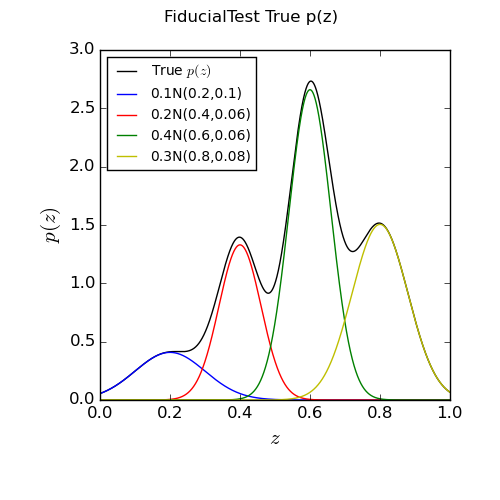
\includegraphics[width=0.5\textwidth]{figs/null/physPz.png}
\caption{The physically-motivated true redshift distribution (black line) used 
in the mock data tests is a sum of Gaussians chosen to have recognizable 
features of different scales so the quality of recovery can be easily 
determined.  The colored curves represent individual Gaussian components each 
with a mean, standard deviation, and relative magnitude.}
\label{fig:physpz}
\end{figure}

The catalog of $J$ photo-z likelihoods $p(\vec{d}_{j}|z_{j})$ is chosen to be a 
set of Gaussian distributions, truncated to the redshift range over which 
$N(z)$ is defined, because it is the simplest extension of the standard 
redshift point estimates with reported error bars.  To obtain the standard 
deviations $\sigma_{j}\sim\mathcal{N}(g\bar{\Delta},(g\bar{\Delta})^{2})$ 
associated with each surveyed galaxy $j$, we first sample a Gaussian 
distribution with mean and standard deviation equal to $g\bar{\Delta}$ for some 
factor $g$ (by default set to unity), truncated to enforce positive standard 
deviations.  Each Gaussian is centered at an "observed" redshift 
$z'_{j}\sim\mathcal{N}(z^{0}_{j},\sigma_{j})$ separated from the true redshift 
$z^{0}_{j}$ by a Gaussian random variable 
$\epsilon_{j}\sim\mathcal{N}(0,\sigma^{2}_{j})$ selected from a distribution of 
mean of 0 and true standard deviation $\sigma_{j}$.   This prescription may be 
understood as an exposition of the generative model of Eq. \ref{eq:genmod} for 
the physically-motivated process originating the data, which states that the 
MLE $z'_{j}$ of the redshift is equal to the true redshift $z^{0}_{j}$ plus a 
Gaussian random variable $\epsilon_{j}$.

\begin{eqnarray}
\label{eq:genmod}
z'_{j} &=& z^{0}_{j}+\epsilon_{j}
\end{eqnarray}

We must also choose the parametrization of the redshift distribution function, 
in this case $f_{\vec{\theta}}(z)=\exp[\vec{\theta}]$ (introduced in Sec. 
\ref{sec:prob}).  We next define the elements of $\vec{\theta}$ to be log 
top-hat functions where the hyperparameters $\theta_{k}$ comprising 
$\vec{\theta}$ take values equal to $\ln[\int_{z_{k-1}}^{z_{k}}\ 
f_{\vec{\theta}}(z)\ dz]$.  By default we choose a flat distribution as the 
interim prior, but others will be tested.  (Such a comparison has been executed 
before by \citet{Viironen2015}.)

To obtain the $J$ desired interim photo-z posteriors $p(z_{j}|\vec{d}_{j})$ 
from the photo-z likelihoods $p(\vec{d}_{j}|z_{j})$, we simply apply Bayes' 
rule as in Eq. \ref{eq:likpost}, where the prior on redshift is 
$p(z_{j}|\vec{\theta}^{0})$ for interim prior $\vec{\theta}^{0}$.  There are 
two unknown constants of proportionality (the likelihood of the data 
$p(\vec{d}_{j})$ and $J$) that we may normalize out according to Eq. 
\ref{eq:norm}.  A random sampling of such interim redshift posteriors is shown 
in Fig. \ref{fig:nullpzs}.

\begin{eqnarray}
\label{eq:likpost}
p(z_{j}|\vec{d}_{j}) &\propto& p(\vec{d}_{j}|z_{j})\ p(z_{j}|\vec{\theta}^{0})
\end{eqnarray}

\begin{eqnarray}
\label{eq:norm}
p(B^{k}_{j}|\vec{d}_{j}) &=& \frac{\int_{z_{k-1}}^{z_{k}}\ 
p(\vec{d}_{j}|z_{j})\ \exp[\vec{\theta}^{0}]\ dz_{j}}{\int_{z_{min}}^{z_{max}}\ 
p(\vec{d}_{j}|z_{j})\ \exp[\vec{\theta}^{0}]\ dz_{j}}
\end{eqnarray}

\begin{figure}
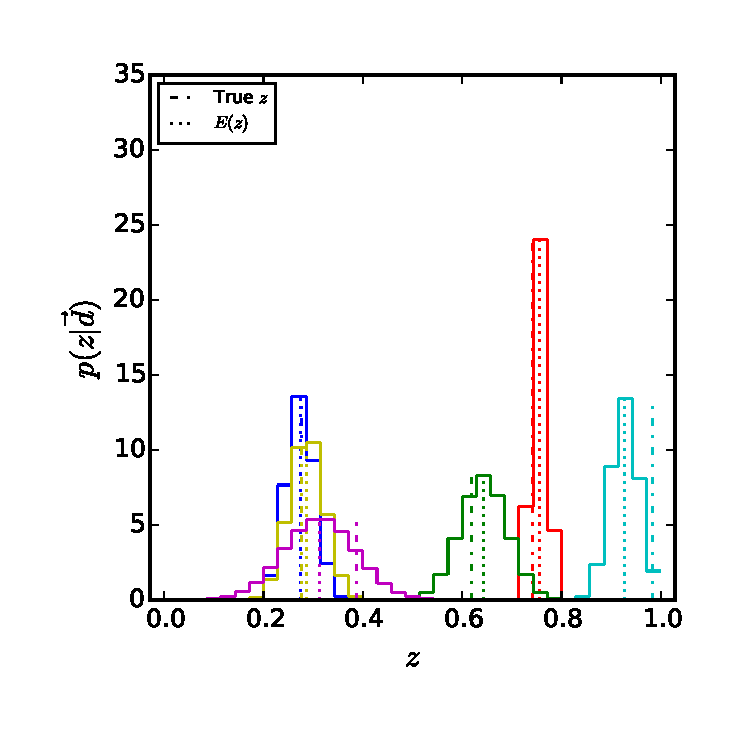
\includegraphics[width=0.5\textwidth]{figs/null/samplepzs.pdf}
\caption{Several examples of individual photo-z posteriors are shown in colors. 
 The simplest case outlined here has likelihoods comprised of a single, 
relatively narrow, Gaussian distribution with a known standard deviation 
centered at a shifted redshift (dotted lines) separated from the true redshift 
(dashed lines) by a Gaussian random variable with the same standard deviation.}
\label{fig:nullpzs}
\end{figure}

\clearpage
\subsubsection{BOSS Data}
\label{sec:data}

We also test this method on subsets of the published interim photo-z posteriors 
of SDSS III DR 10.  A sampling of the provided interim photo-z posteriors of 
dimension $K=35$ for $z_{min}=0.3$ and $z_{max}=1.4$ is shown in Fig. 
\ref{fig:datapzs}.  The interim prior used for this set of interim redshift 
posteriors is the reweighted estimator of $N(z)$ of \citet{Sheldon2012}.

\begin{figure}
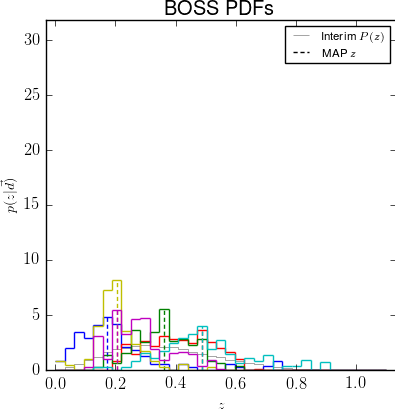
\includegraphics[width=0.5\textwidth]{figs/boss/samplepzs.png}
\caption{Pictured here are examples of actual photo-z posteriors produced by 
\citet{Sheldon2012}.  It can be seen that the real data is much more structured 
than the simulated data of Fig. \ref{fig:nullpzs}.}
\label{fig:datapzs}
\end{figure}

\clearpage
\subsection{Computation}
\label{sec:mcmc}

The testing procedure is implemented in \texttt{Python}.  The code takes as 
input a \texttt{csv} file containing the basis for the binning of redshift 
space, a specification of the interim prior $\vec{\theta}^{0}$, and a catalog 
of $J$ interim photo-z log-posteriors 
$\{\ln[p(B_{j}|\vec{d}_{j},\vec{\theta}^{0})]\}_{J}$.

The \texttt{emcee} \citep{Foreman-Mackey2013} implementation of ensemble 
sampling is applied to sample the full posterior of Eq. \ref{eq:final}.   For 
each of some $W$ walkers at each iteration $i$, a proposal distribution 
$\vec{\theta}^{i}$ generated from the hyperprior distribution and evaluated for 
acceptance to or rejection from the desired posterior distribution.  % 
according to the algorithm outlined below.  
%
%\begin{enumerate}
%\item \label{it:randsamp} Sample the hyperprior $\ln[p(\vec{\theta})]$ to 
generate a proposal $\vec{\theta}^{i}$.
%\item Calculate the log posterior as in Eq. \ref{eq:final} to produce a 
quantity proportional to $\ln[p(\vec{\theta}^{i}|\{\vec{d}_{j}\}_{J})]$.
%\item Calculate 
$a=\ln[p(\vec{\theta}^{i}|\{\vec{d}_{j}\}_{J})]-\ln[p(\vec{\theta}|\{\vec{d}_{j}
\}_{J})]$.
%\item If $a\geq0$, set and record $\vec{\theta}=\vec{\theta}^{i}$.\\
%If $a<0$, select a random number $n$ from the uniform distribution between 0 
and 1.
%\begin{enumerate}
%\item If $n<\exp[a]$, set and record $\vec{\theta}=\vec{\theta}^{i}$.
%\end{enumerate}
%\item Check if the threshold condition has been achieved; if not, return to 
Step \ref{it:randsamp}.
%\end{enumerate}
Two threshold conditions are defined, one designating all previous samples to 
be ignored as as products of a "burn-in" phase and another indicating when a 
sufficient number of "post-burn" samples have been accepted.  In this case, the 
first threshold (described in Sec. \ref{sec:acorr}) is defined in terms of 
sub-runs of $I_{0}=100$ accepted samples, and the second is defined as an 
accumulation of an arbitrary 6000 samples.

The input/output format chosen for this work is \texttt{HDF5} because of its 
efficiency for large amounts of data.  The resulting output is a set of $I$ 
ordered \texttt{hickle} files enumerated by $\rho$ containing the state 
information after each sub-run.  The state information includes 
$\frac{I_{0}}{s}$ actual samples $\vec{\theta}^{i}$ for a pre-specified chain 
thinning factor $s$ and their full posterior probabilities 
$p(\vec{\theta}^{i}|\{\vec{d}_{j}\}_{J})$ as well as the autocorrelation times 
and acceptance fractions calculated for each element of $\vec{\theta}$ over the 
entire sub-run.  

\clearpage
\subsubsection{Prior}
\label{sec:prior}

The method described above involves the assumption of a hyperprior distribution 
$p(\vec{\theta})$ over the hyperparameters comprising $\vec{\theta}$.  The 
prior chosen here is a multivariate normal distribution with mean 
$\vec{\theta}^{0}$ equal to the interim prior and covariance $\textul{\Sigma}$ 
inspired by one used in Gaussian processes, given by Eq. \ref{eq:priorcov}.  
This choice is made to permit draws from this prior distribution to produce 
shapes similar to that of the true $\tilde{\theta}$.  Here, the parameters of 
this covariance matrix are set to the small numbers $q=1.0$, $e=100.0$, and 
$t=q\cdot10^{-5}$.  We adapt the full posterior of Eq. \ref{eq:final} to the 
binning of redshift space chosen in Sec. \ref{sec:mock}.

\begin{eqnarray}
\label{eq:priorcov}
\Sigma_{a,b} &=& q\ \exp[-\frac{e}{2}\ (\bar{z}_{a}-\bar{z}_{b})^{2}]\ +\ 
t\delta(a,b)%\ \mathbb{I}_{a,b}
\end{eqnarray}

The sampler is initialized with $W=100$ walkers each with a value chosen from a 
Gaussian distribution of identity covariance around a sample from the 
hyperprior distribution.  An example of such samples from the prior are shown 
in Fig. \ref{fig:prior}.

\begin{figure}
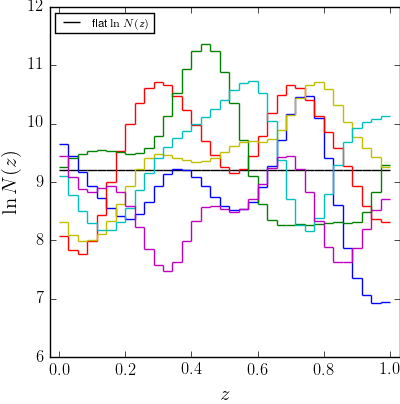
\includegraphics[width=0.5\textwidth]{figs/null/priorsamps.png}
\caption{Samples (colored lines) from the prior distribution with a flat mean 
over $J'=10,000$ galaxies are shown in the figure.}
\label{fig:prior}
\end{figure}

\clearpage
\subsubsection{Convergence Criteria}
\label{sec:acorr}

Two quantities that probe the convergence of the sampler are used in this 
study, the autocorrelation time and the posterior probability evolution.

The autocorrelation time is effectively a measure of the convergence rate of 
the method and can be described as the expected number of iterations necessary 
to accept a new sample independent of the current accepted sample.  A sampler 
that converges faster will have a smaller autocorrelation time, and smaller 
autocorrelation times are preferable because it means fewer iterations are 
wasted on non-independent samples when independent samples are desired.  See 
\citet{Foreman-Mackey2013} for a more complete exploration of the 
autocorrelation time.  Fig. \ref{fig:acorr} shows the behavior of the 
autocorrelation time for a test case representative of all mock data tests.

\begin{figure}
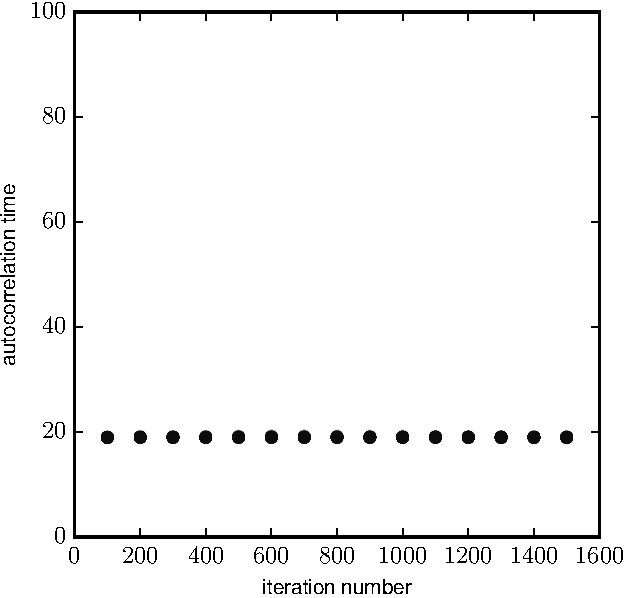
\includegraphics[width=0.5\textwidth]{figs/null/times.pdf}
\caption{The autocorrelation times shown here for the null case are 
representative of all tests on mock data.  Given an accepted sample, the next 
independent accepted sample is approximately twenty accepted samples later.  
The autocorrelation times are plotted here as individual points with one per 
walker.}
\label{fig:acorr}
\end{figure}

We examine the evolution of the posterior probability of accepted samples after 
each successive sub-run to evaluate the duration of the burn-in phase.  Though 
the probability associated with the initial values will likely be quite low, it 
should improve for subsequent accepted parameter values.  As with the 
autocorrelation time, the posterior probability of samples will asymptotically 
approach some more favorable value with more iterations.  This behavior is 
shown in Fig. \ref{fig:probs}.  The burn-in phase may be defined as the number 
of iterations necessary before the variance of the log probabilities is less 
than the change in median log probability over the sub-run.  Samples accepted 
during the burn-in phase are discounted from analysis, and an arbitrary ten 
additional sub-runs are executed before the sampler terminates.  

\begin{figure}
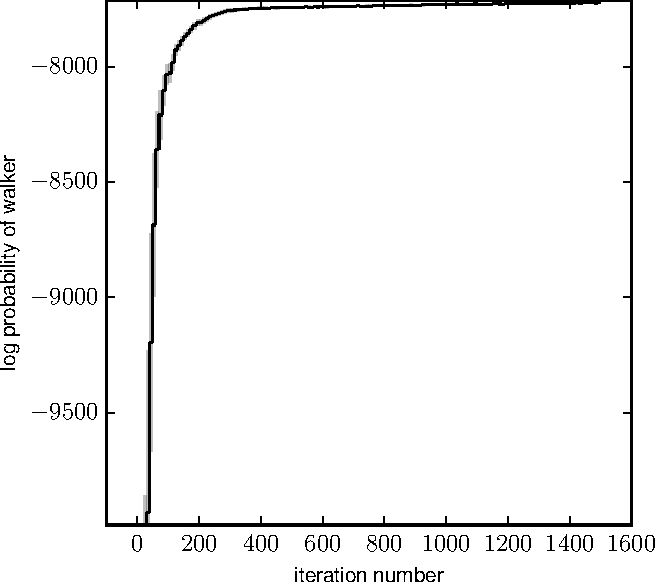
\includegraphics[width=0.5\textwidth]{figs/null/probs.pdf}
\caption{The log-posterior probability evolution of the samples is shown here.  
One can see that the mean (black line) of the log-posterior probability over 
all walkers at a given time step quickly converges as the one and two-sigma 
error regions (dark and light gray regions, respectively) decrease.}
\label{fig:probs}
\end{figure}

\textbf{Is this sufficient discussion of measures of convergence?  Should I 
discuss others, even though these are the only ones I actually used?}

\clearpage
\subsection{Diagnostics}
\label{sec:diag}

The results of the computation described in Sec. \ref{sec:mcmc} are evaluated 
for accuracy on the basis of some quantitative measures.  Beyond visual 
inspection of samples, we calculate summary statistics to quantitatively 
compare different estimators' precision and accuracy.  Since MCMC samples of 
hyperparameters are Gaussian distributions, we can quantify the breadth of the 
distribution for each hyperparameter using the standard deviation regardless of 
whether the true values are known.  

In simulated cases where the true parameter values are known, we calculate the 
Kullback-Leibler divergence (KLD), given in Eq. \ref{eq:kl}, which measures a 
distance between parameter values $\vec{\theta}^{a}$ and $\vec{\theta}^{b}$ 
that is invariant under changes of variables.  We note that $KL_{ab}\neq 
KL_{ba}$, so both must be calculated, and the minimum of the two is reported in 
this study.  In simulated tests, one of $\vec{\theta}^{a}$ and 
$\vec{\theta}^{b}$ is the true value and the other is the value produced by one 
of the methods in question.  

\begin{eqnarray}
\label{eq:kl}
KL_{ab} &=& \sum_{k=1}^{K}\ \exp[\theta_{k}^{a}]\ 
\ln\left[\frac{\theta_{k}^{a}}{\theta_{k}^{b}}\right]\ \Delta_{k}
\end{eqnarray}

%The mean squared error of samples may also be calculated.  If there is a 
strongly peaked distribution of values for a parameter, it ought to peak close 
to the true value (and is in fact guaranteed to asymptotically approach the 
marginalized maximum likelihood value) if we are to conclude that the sampler 
is successful; if the distribution is broad, it may reflect inherent 
uncertainty in inferring the hyperparameters.

\clearpage
\section{Validation Tests}
\label{sec:valid}

\textbf{This is the section that's weakest, and, I am aware, also the most 
important.  I could use some concrete recommendations of how to change it to be 
publishable.}

Here we motivate and present the results of several informative tests.  The 
code was tested on simulated datasets each of size $J'=10,000$.  The fiducial 
experiment of Sec. \ref{sec:null} was generated by code following the procedure 
given in Sec. \ref{sec:mock}.  Seven other cases vary the shapes of the photo-z 
likelihoods (Secs. \ref{sec:noisy} and \ref{sec:unc}), the true redshift 
distribution function (Sec. \ref{sec:fake}), and the interim prior (Sec. 
\ref{sec:interim}).  Two additional cases with SDSS-III BOSS data described in 
Sec. \ref{sec:data} are also considered.  A summary of all KLD values is given 
in Tab. \ref{tab:kld}, with the best fit estimator in bold.

\begin{table}
\begin{tabular}{lccccc}
& Mean of & Marginalized & Stacking & Marginalized & Marginalized\\
& Samples & MLE & & MAP & Expected Value\\
Fiducial &&&&&\\
Doubly Imprecise Likelihoods &&&&&\\
Quadruply Imprecise Likelihoods &&&&&\\
Inaccurate Likelihoods &&&&&\\
Multimodal Likelihoods &&&&&\\
Toy Model True $N(z)$ &&&&&\\
Low-$z$ Favoring Interim Prior &&&&&\\
Mid-$z$ Disfavoring Interim Prior &&&&&\\
BOSS Data &&&&&\\
Biased BOSS Data &&&&&\\
\end{tabular}
\caption{}
\label{tab:kld}
\end{table}

\clearpage
\subsection{Fiducial Case}
\label{sec:null}

For the fiducial experiment, we precisely follow the procedures outlined in 
Sec. \ref{sec:mock} and Sec. \ref{sec:mcmc}.  Fig. \ref{fig:null-samp} shows 
some random sample values, the true value of $N(z)$.  Fig. \ref{fig:null-comp} 
compares the mean of the sample values to alternative estimators as well as the 
truth.

\begin{figure}
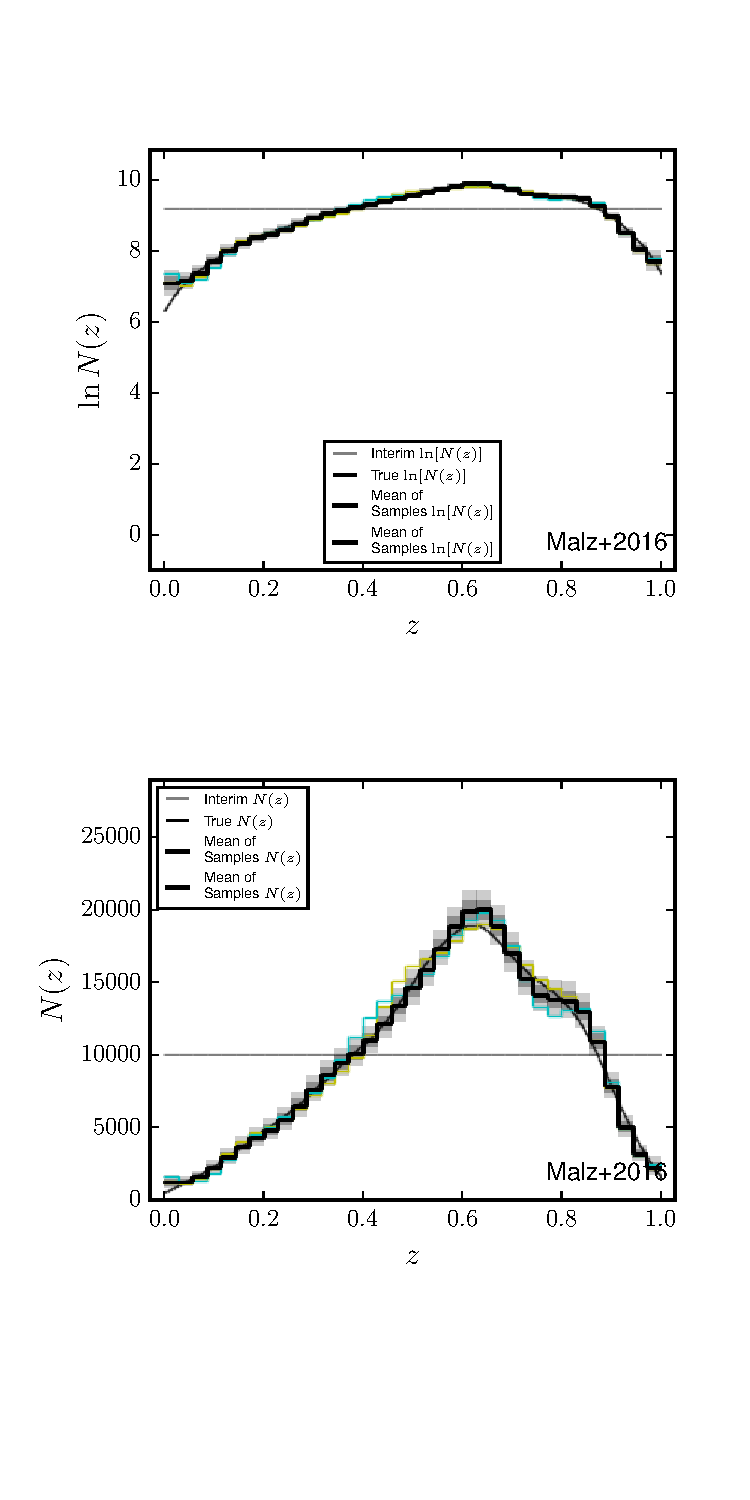
\includegraphics[width=0.5\textwidth]{figs/null/samps.pdf}
\caption{This test was conducted with a flat interim prior (gray line) and 
produced a mean of samples (thick, black line) that accurately reproduces the 
truth.  It can be seen that the samples (colored lines) are an excellent 
estimator of the true $N(z)$ (thin, black line) with the true values falling 
within the error bars ($1\sigma$ in dark gray, $2\sigma$ in light gray).}
\label{fig:null-samp}
\end{figure}

\begin{figure}
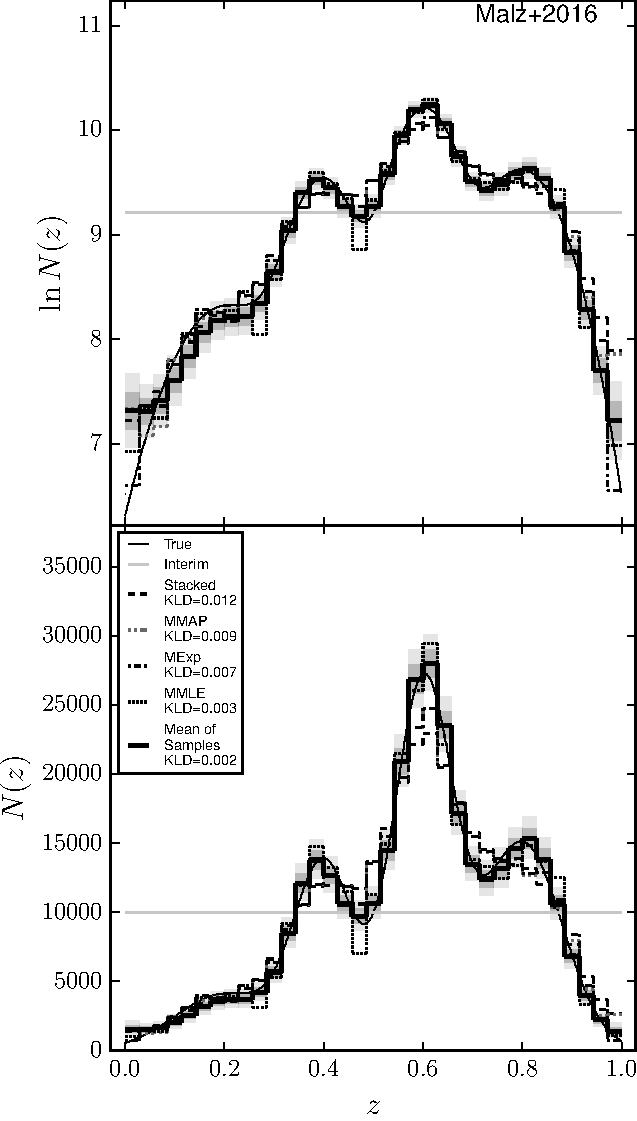
\includegraphics[width=0.5\textwidth]{figs/null/comps.pdf}
\caption{It can be seen that the mean of the samples (thick, black line) is a 
better estimator of the true distribution (thin, black line); stacking (dotted 
line) overestimates $N(z)$ at the tails and underestimates $N(z)$ at the peaks, 
and marginalized likelihood maximization (dashed line) is unstable.}
\label{fig:null-comp}
\end{figure}

In the fiducial case, hierarchical inference preserves features in the redshift 
distribution function, whereas stacking tends to smear them out.  The 
difference between stacking and the mean of the samples is more evident in 
cases of noisier data, discussed in Sec. \ref{sec:noisy}.

\clearpage
\subsection{Imprecise interim photo-z posteriors}
\label{sec:noisy}

Several factors contribute to photometric redshifts' intrinsic scatter.  
Distant galaxies are dimmer compared to galaxies of identical luminosity that 
are closer, driving up photometric errors in flux-limited surveys.  The nature 
of the galaxy sample at higher redshifts also changes, meaning the generation 
of the photometric redshift posterior based on an a locally-calibrated SED 
template library or spectroscopically-confirmed training is more likely to be 
inappropriate, leading to broader features.

Here we vary the fiducial case with noisier data to demonstrate that the 
results of the sampler and of stacking diverge for broader photo-z likelihoods. 
 In these cases, $\sigma_{j}$ is drawn from a normal distribution as described 
in Sec. \ref{sec:mock} but with the factor $f=2$ in one case and $f=4$ in 
another.  \textbf{Should I even mention the $f=2$ case?  It's not nearly as 
dramatic.}  In both cases, the corresponding sample interim photo-z posteriors 
to those of Fig. \ref{fig:nullpzs} are broader, with central redshifts farther 
from the true redshift on average.  \textbf{I cut the figure since I think this 
sentence suffices.}

%\begin{figure}
%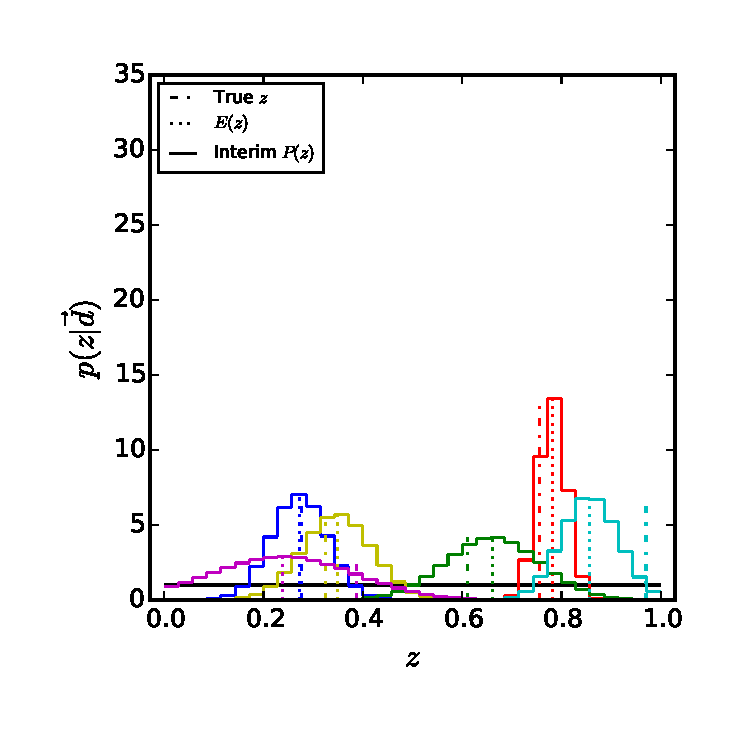
\includegraphics[width=0.5\textwidth]{figs/sig2/samplepzs.pdf}
%\caption{The interim photo-z posteriors (colored lines) here have the same 
true redshifts (dotted lines) and means of the distribution (dotted lines) as 
those of Fig. \ref{fig:nullpzs} but have two times the standard deviation.}
%\label{fig:sig2pzs}
%\end{figure}
%
%\begin{figure}
%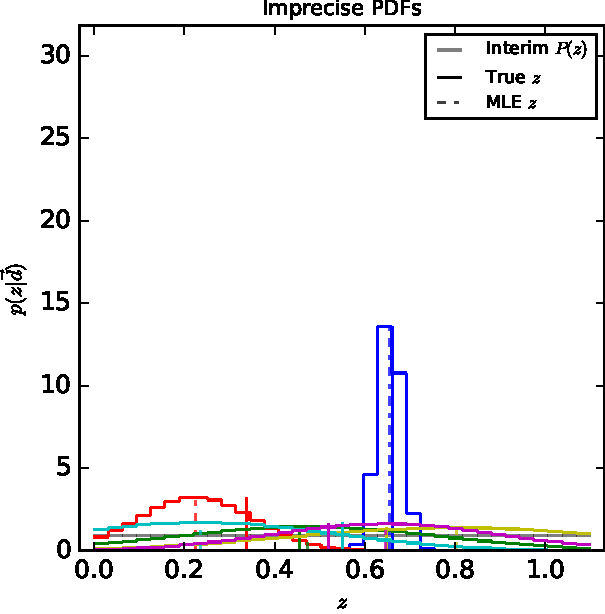
\includegraphics[width=0.5\textwidth]{figs/sig4/samplepzs.pdf}
%\caption{The interim photo-z posteriors (colored lines) here have the same 
true redshifts (dotted lines) and means of the distribution (dotted lines) as 
those of Fig. \ref{fig:nullpzs} but have four times the standard deviation.}
%\label{fig:sig4pzs}
%\end{figure}

The sampler was run on these two, noisier datasets with broader likelihoods and 
produced broader error bars on the mean of the samples, with little effect on 
the value of the mean of the samples.  Fig. \ref{fig:sig4-comp} shows this 
result for the $f=4$ case.  The alternative methods are more strongly affected 
by the broadened likelihoods; as the standard deviation of the photo-z 
likelihood functions increases, the stacked result becomes so broad as to erase 
all features from the estimate of $N(z)$, while the marginalized MLE enhances 
peaks and troughs to bias the estimate.

%\begin{figure}
%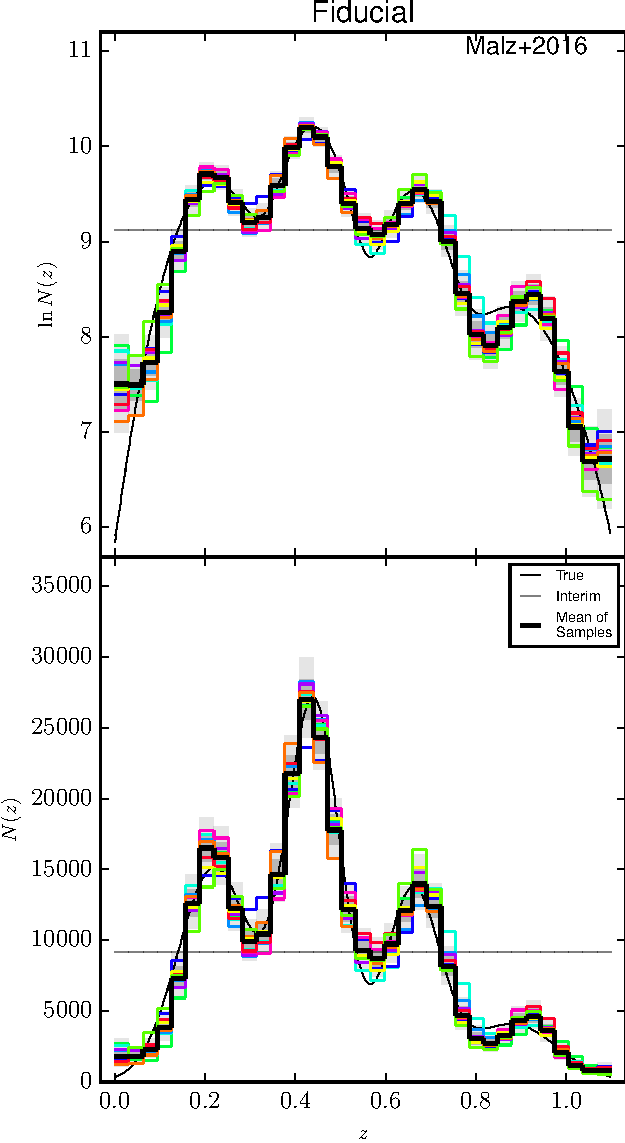
\includegraphics[width=0.5\textwidth]{figs/sig2/samps.pdf}
%\caption{The mean of sampled values (thick, black line) is quite comparable to 
that of the original fiducial case even though the data is twice as noisy.  
However, the error bars ($1\sigma$ in dark gray, $2\sigma$ in light gray) are 
somewhat larger.}
%\label{fig:sig2-samp}
%\end{figure}
%
%\begin{figure}
%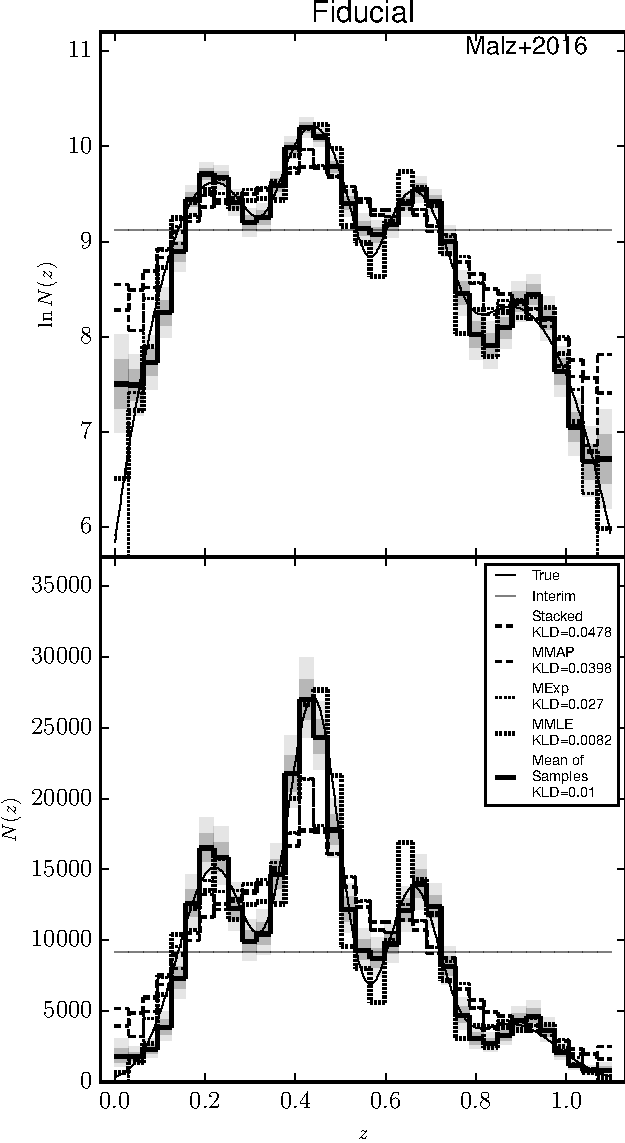
\includegraphics[width=0.5\textwidth]{figs/sig2/comps.pdf}
%\caption{The mean of sampled values (thick, black line) is prone to 
overestimating the peak values and underestimating the trough values relative 
to the true $N(z)$ (thin, black line).  The result of stacking (dotted line), 
on the other hand, underestimates the peak values, overestimates the trough 
values, and increases the weight of the tails, leading to a greater KLD than 
for the sampler.  The marginalized MLE (dashed line) performs well, but is more 
prone to the biases that affect the sampler, so has a larger KLD than the 
sampler as well.}
%\label{fig:sig2-comp}
%\end{figure}
%
%\begin{figure}
%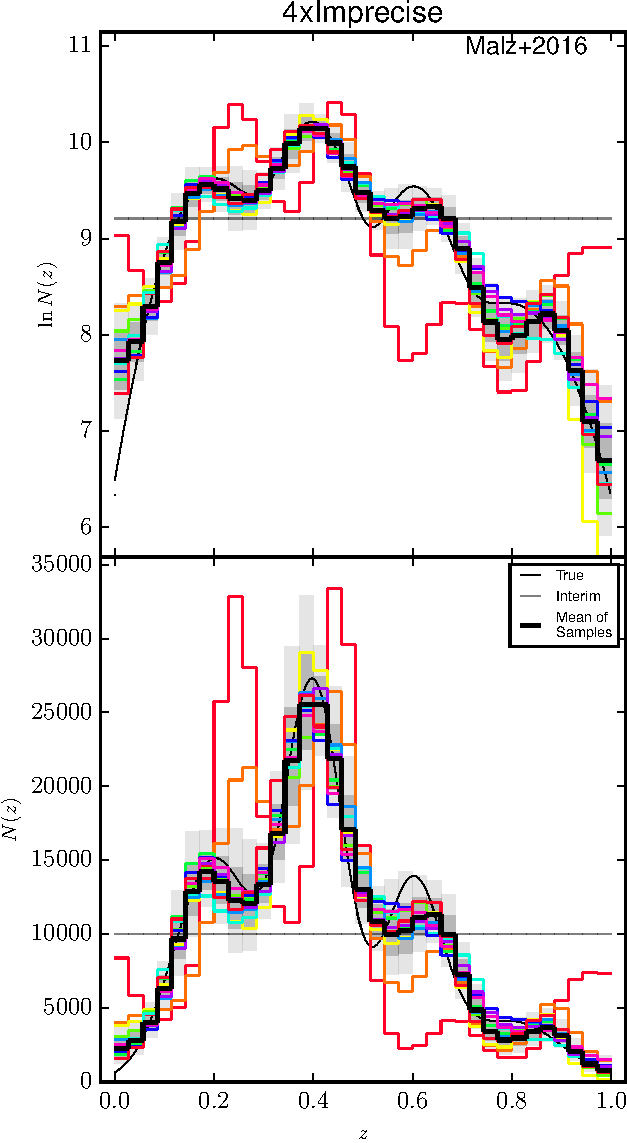
\includegraphics[width=0.5\textwidth]{figs/sig4/samps.pdf}
%\caption{Compared to Fig. \ref{fig:null-samp}, the greatest difference between 
the original fiducial case and the quadruply noisy case is the size of the 
error bars ($1\sigma$ in dark gray, $2\sigma$ in light gray) about the true 
$N(z)$ (thin, black line), as exemplified by the plotted random samples 
(colored lines) that scatter further from the mean of the sampled values 
(thick, black line).}
%\label{fig:sig4-samp}
%\end{figure}

\begin{figure}
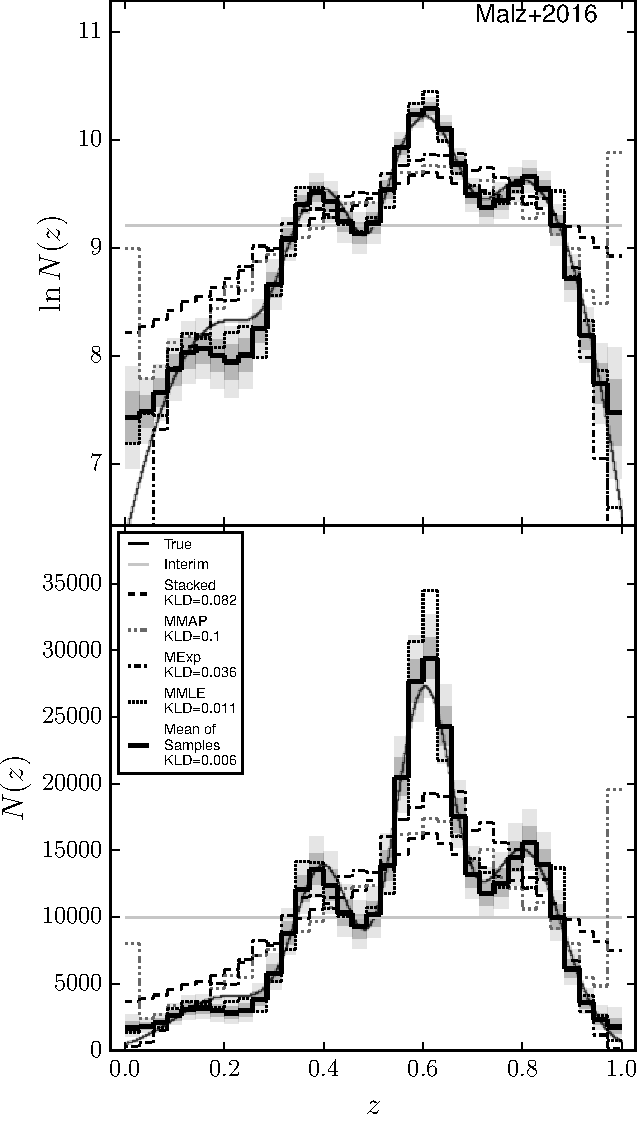
\includegraphics[width=0.5\textwidth]{figs/sig4/comps.pdf}
\caption{Here it is most obvious that stacking (dotted line) erases features 
from an estimate of the true $N(z)$ (thin, black line).  The mean of sampled 
values (thick, black line) does exhibit some bias at the peaks and troughs of 
the distribution, but it overall performs better than the stacked estimator and 
the marginalized MLE (dashed line).}
\label{fig:sig4-comp}
\end{figure}

\clearpage
\subsection{Inaccurate interim photo-z posteriors}
\label{sec:multi}

\textbf{Should I cut these two tests out of the paper?  Both violate the 
generative model, which is kind of the point.  I'm just not confident in my 
interpretation of the biases of the results of sampling.}

In this pair of tests, we aim to simulate more realistic interim photo-z 
posteriors by modifying the procedure of Sec. \ref{sec:mock} to introduce 
inaccuracy that causes catastrophic photo-z errors.  Catastrophic photo-z 
errors arise from a degeneracy in the space of galaxy SEDs and redshifts, 
wherein a galaxy of one SED type at one redshift has photometry 
indistinguishable from a galaxy of another SED type at another redshift.  In 
this case, the Gaussian components of the likelihood may have standard 
deviations that do not correspond to the true standard deviation used to 
generate the data, or there may be multiple components to the interim photo-z 
posteriors.  Both cases will be considered here by introducing one change in 
the steps of Sec. \ref{sec:mock}.  

The first case modifies the generative model of Eq. \ref{eq:genmod} is modified 
to have $\epsilon_{j}\sim\mathcal{N}(0,\sigma'^{2}_{j})$ for 
$\sigma'_{j}\sim\mathcal{N}(\bar{\Delta},\bar{\Delta}^{2})$.  The mean of the 
sampled hyperparameter values is compared to the results of stacking and other 
alternatives in Fig. \ref{fig:noisy-comp}.  It can be seen that inaccurate 
interim photo-z posteriors are best handled by the sampler, whose KLD is lower 
than that of stacking and marginalized likelihood maximization.

%\begin{figure}
%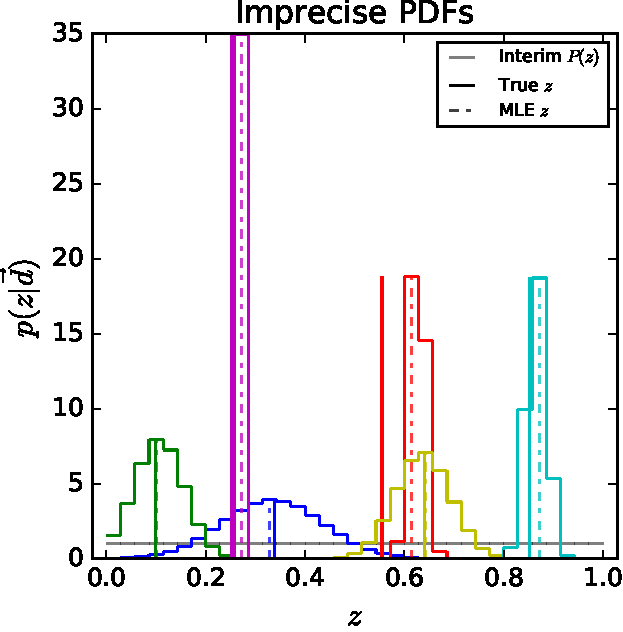
\includegraphics[width=0.5\textwidth]{figs/vars/samplepzs.pdf}
%\caption{Several examples of noisified individual interim photo-z posterior 
distributions (colored lines) are shown with their true redshifts (dotted 
lines) and the central redshift of the distribution (dotted lines).  Note that 
the widths of the Gaussians vary randomly over the samples and do not 
necessarily correlate with redshift.}
%\label{fig:noisypzs}
%\end{figure}
%
%\begin{figure}
%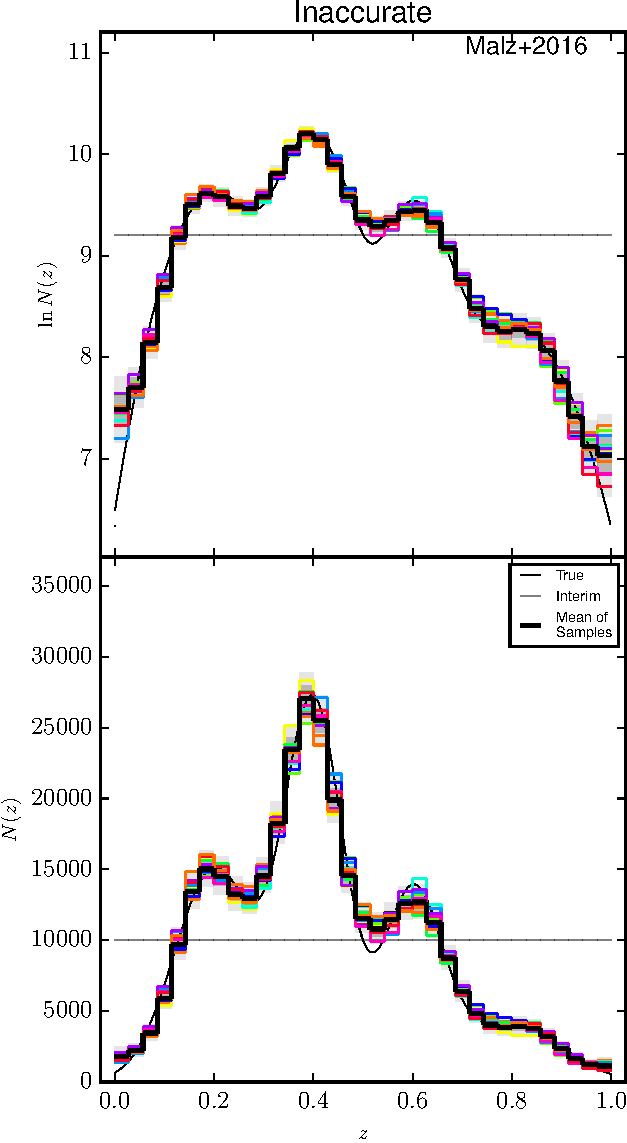
\includegraphics[width=0.5\textwidth]{figs/vars/samps.pdf}
%\caption{The mean of the sampled values (thick, black line) accurately 
reproduces the true $N(z)$ distribution (thin, black line) such that the true 
values always fall within the error bars ($1\sigma$ in dark gray, $2\sigma$ in 
light gray).  Some samples (colored lines) are shown as well.}
%\label{fig:noisy-samp}
%\end{figure}

\begin{figure}
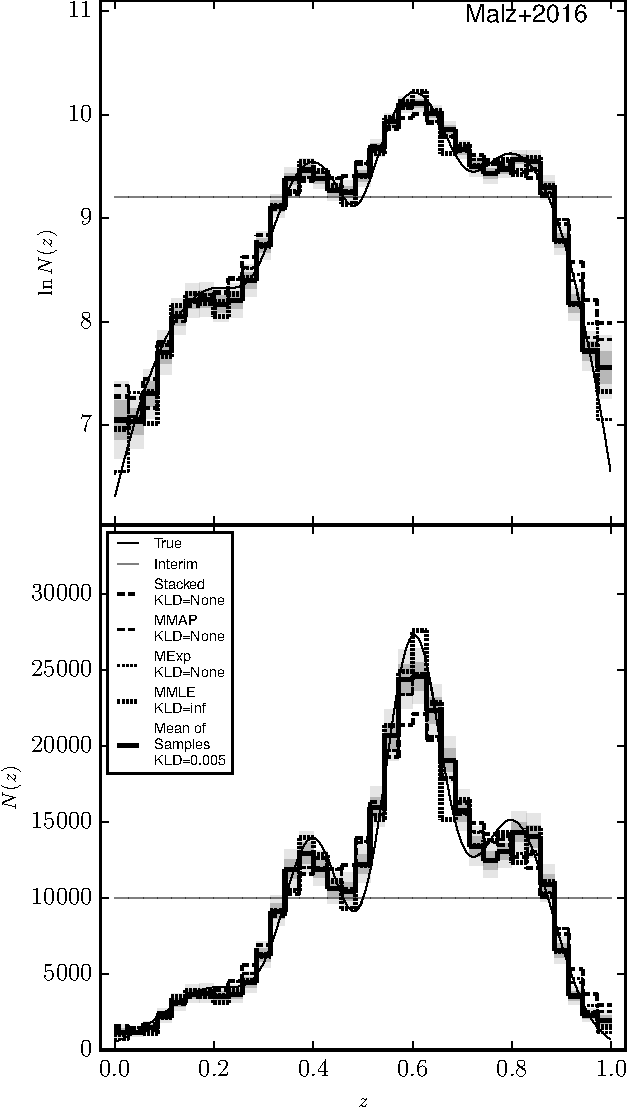
\includegraphics[width=0.5\textwidth]{figs/vars/comps.pdf}
\caption{The result of the sampler (thick, black line), like the marginalized 
MLE (dashed line), does have a bias to overestimate density in the peaks and 
underestimate it in the troughs.  However, the effect is not as severe as for 
the result of stacking (dotted line), which smooths out all features and 
increases probability density in the tails.}
\label{fig:noisy-comp}
\end{figure}

In the second test case, inaccuracy is simulated by considering multimodal 
photo-z likelihoods.  To achieve this goal we introduce another change in Sec. 
\ref{sec:mock}.  Here, the redshift posteriors are sums of Gaussians of the 
form of those tested in Sec. \ref{sec:null}.  Each galaxy is assigned a number 
$R_{j}$ of Gaussian elements to be summed, chosen randomly from $1,\dots,K$ 
with weights proportional to $K^{-1}$.  One $\sigma_{jr}$ is drawn for each 
$r=1,\dots,R_{j}$, and one $z'_{jr}$ is selected from the corresponding 
$\mathcal{N}(z^{0}_{j},\sigma^{2}_{jr})$.  The components are summed and 
normalized to yield the likelihood, which is then convolved with the interim 
prior to produce the interim posterior.  Some examples of the multimodal 
interim photo-z posteriors are shown in Fig. \ref{fig:multipzs}.  \textbf{I 
redid this test with fewer summed components, but they're still not multimodal, 
just asymmetric.  This is because the generative model doesn't let the peaks be 
far enough apart relative to their variances.  Unless I violate the generative 
model as in the previous case, I should probably cut this test out of the 
paper.}

\begin{figure}
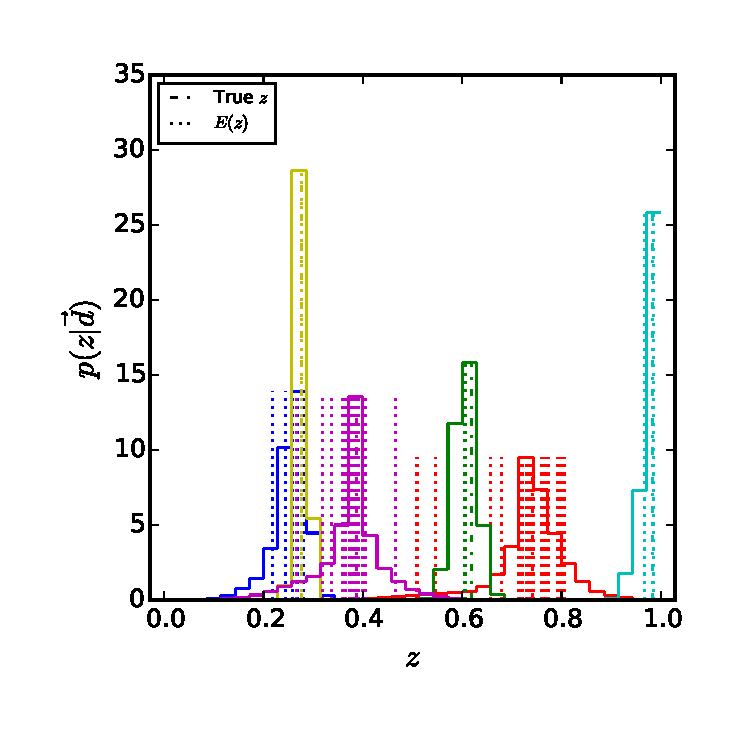
\includegraphics[width=0.5\textwidth]{figs/mult/samplepzs.pdf}
\caption{Several examples of individual interim photo-z posteriors (colored 
lines) are shown, along with the true redshift (dashed lines) and the $R_{j}$ 
centers of the Gaussian components (dotted lines).  Note that some 
distributions are multimodal, with peaks of different heights, while others are 
simply asymmetric in spite of the flat interim prior.}
\label{fig:multipzs}
\end{figure}

Fig. \ref{fig:multi-comp} shows a comparison to alternative methods.  It can be 
seen that the lessened quality of the data does impact the accuracy of the mean 
of the posterior samples as an estimator of the truth, exaggerating the signal 
at the peaks and troughs.  However, the alternatives do worse as measured by 
the KLD, with stacking smoothing the peaks and troughs.

%\begin{figure}
%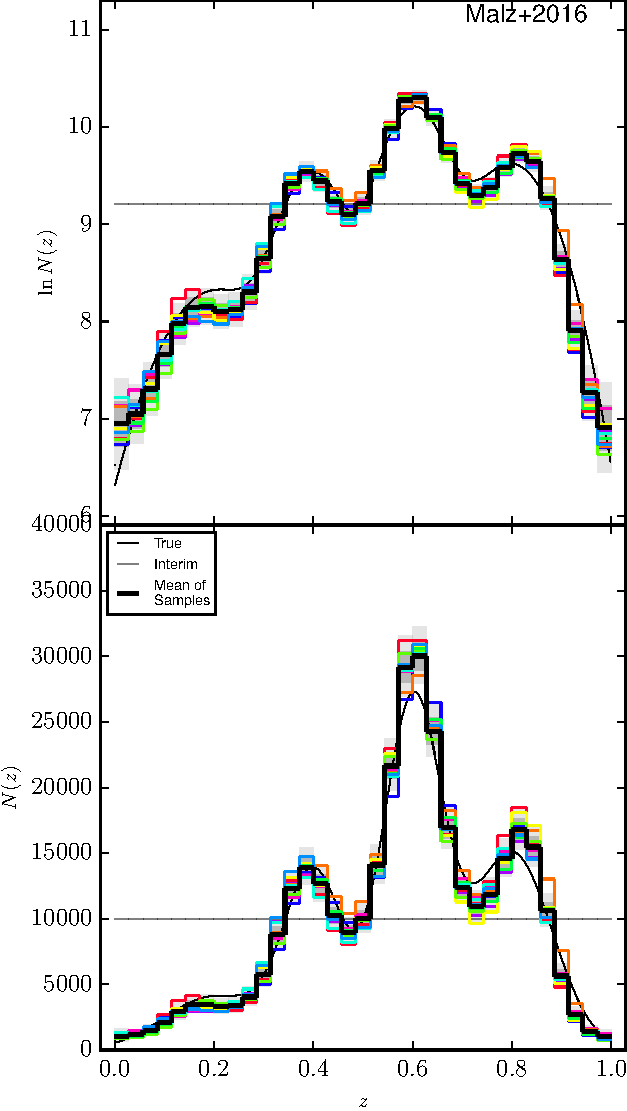
\includegraphics[width=0.5\textwidth]{figs/mult/samps.pdf}
%\caption{The mean of the sampled values (thick, black line) appears to do a 
relatively poor job of recovering the true $N(z)$ (thin, black line), enhancing 
peaks and troughs compared to the true distribution and underestimating the 
probability density in the tails.  The samples (colored lines) are quite close 
to the mean with error bars ($1\sigma$ in dark gray, $2\sigma$ in light gray) 
tight enough to exclude the true value.}
%\label{fig:multi-samp}
%\end{figure}

\begin{figure}
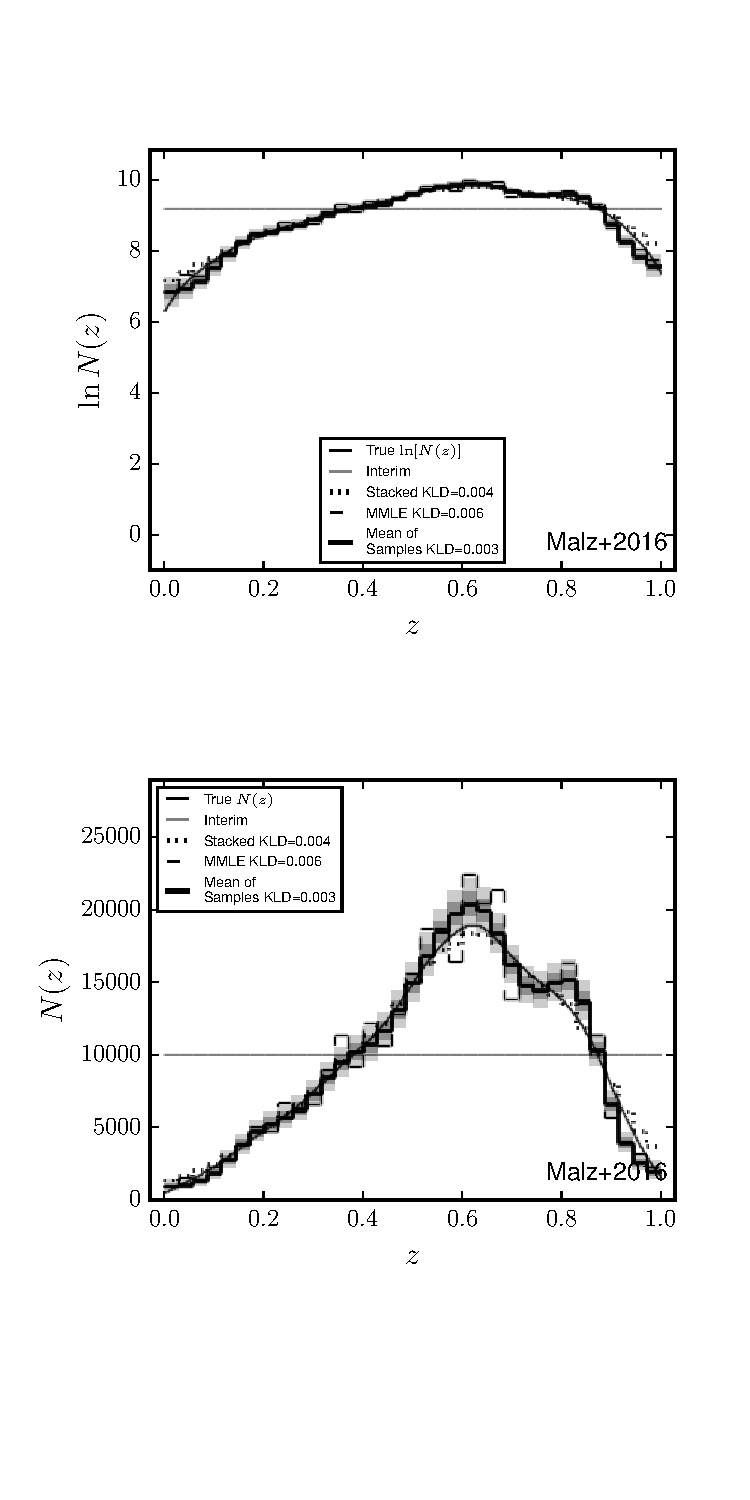
\includegraphics[width=0.5\textwidth]{figs/mult/comps.pdf}
\caption{Though the sampler (thick, black line) fails to recover the true 
$N(z)$ (thin, black line), it still does better than stacking (dotted line) and 
marginalized likelihood maximization (dashed line).  It is less unstable than 
the marginalized MLE and displaces less probability density at the tails than 
stacking.}
\label{fig:multi-comp}
\end{figure}

\clearpage
\subsection{Toy Model $N(z)$}
\label{sec:fake}

We test the sampler in a case of a highly unrealistic but strongly featured 
true $N(z)$.  This is done to show that the sampler works even in extreme and 
unanticipated conditions.  Instead of sampling the physically motivated true 
distribution $p(z|\vec{\theta}')$ as in Sec \ref{sec:mock}, we assign all 
galaxies the same true redshift.  Further, the prior is taken to have identity 
covariance instead of that of Sec. \ref{sec:prior}.  

Fig. \ref{fig:toy-comp} compares the mean of the posterior samples to the 
results of stacking and marginalized likelihood maximization.  It can be seen 
that the marginalized maximum likelihood estimator is best at recovering the 
true distribution of a delta function, whereas stacking and the point 
estimators broaden it considerably.  The sampler does a fair job of recovering 
the true distribution, with minimal broadening.

%\begin{figure}
%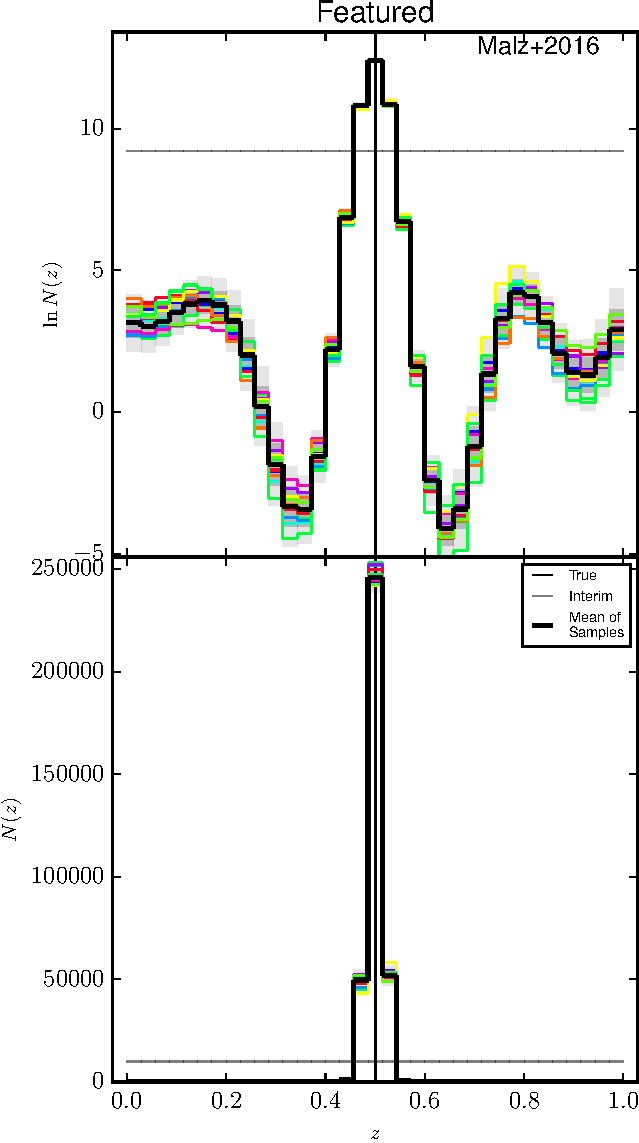
\includegraphics[width=0.5\textwidth]{figs/delt/samps.pdf}
%\caption{}
%\label{fig:toy-samp}
%\end{figure}

\begin{figure}
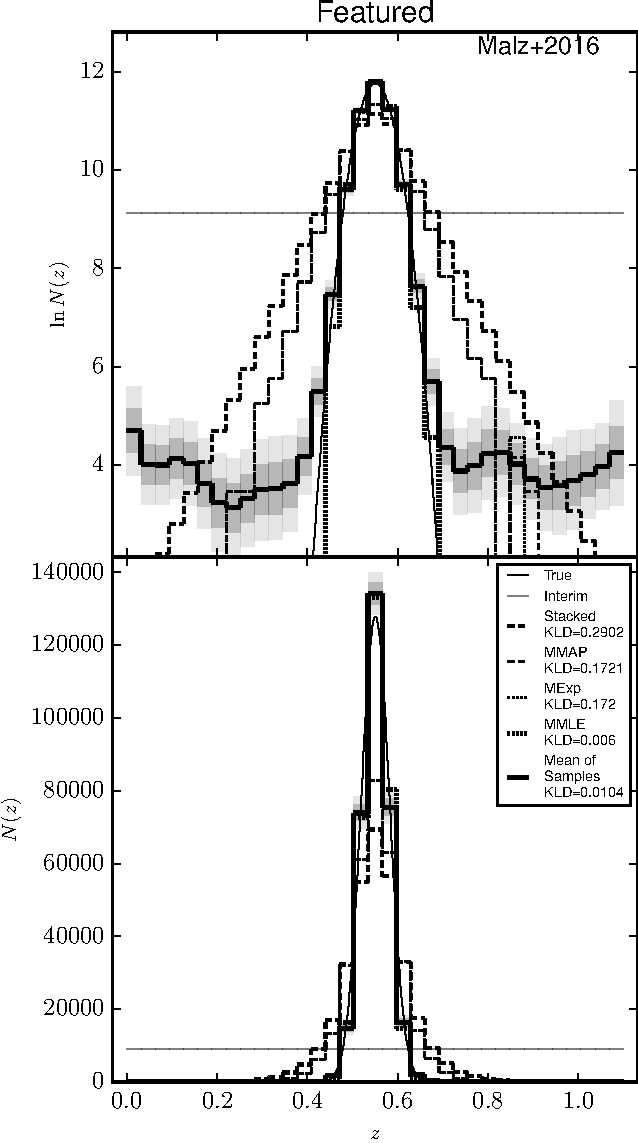
\includegraphics[width=0.5\textwidth]{figs/delt/comps.pdf}
\caption{In this case, the underlying $N(z)$ is a delta function, but the KDE 
of the true redshift values is a narrow Gaussian.  The sampler (thick, black 
line) and marginalized MLE (dark dot-dashed line) recover the underlying $N(z)$ 
but not the true $N(z)$ (thin, black line).  The results of stacking (dotted 
line) and the point estimators estimate very broad $N(z)$ parameters that .  It 
is less unstable than the marginalized MLE and displaces less probability 
density at the tails than stacking.}
\label{fig:toy-comp}
\end{figure}

\clearpage
\subsection{Variable Interim Prior}
\label{sec:interim}

In the following two cases we vary the interim prior used in Sec. 
\ref{sec:mock} to show that the sampler is robust to inappropriate choices of 
interim prior so long as that interim prior is known.  Typically, interim 
redshift posteriors are made with an interim prior derived from $N(z)$ in a 
previous observational study.  Since most observational studies used for this 
purpose are spectroscopically confirmed and objects for which photometric 
redshifts are relied upon make up a population that cannot be spectroscopically 
confirmed, such an interim prior is rarely appropriate.  Some efforts have been 
made to modify an observationally informed interim prior so that it is more 
representative of the data set.  \citep{Sheldon2012}  However, any interim 
prior of this kind imparts information into the interim redshift posteriors.  
Ideally, an uninformative interim prior would be used, although it may be 
complicated to compute from the covariances of the raw data.  In this test, we 
consider two obviously inappropriate interim priors and compare the result to 
that of the flat interim prior used in previous tests according to Sec. 
\ref{sec:mock}.

In some cases, the interim prior is chosen to be the final product of a 
previously conducted spectroscopic redshift survey.  Because low-redshift 
galaxies are more likely to be bright enough to be observed by such a survey, 
$N(z)$ determined from that sample may be heavily biased to low redshift 
galaxies.  By contrast, the galaxies that were unobserved in such a survey are 
more likely be dimmer, making them more likely to be at higher redshifts.  
Since the interim prior is not compatible with our beliefs about the true 
redshift distribution, the resulting interim redshift posteriors will be 
inappropriate.  In this test, we choose an interim prior with most of its 
weight at low redshifts and observe its influence on the recovery of the true 
$N(z)$ by different methods.  

A comparison of the sampler to other approaches is shown in Fig. 
\ref{fig:intu-comp}.  It can be seen that the mean of the samples has a lower 
KLD than the result of stacking.

%\begin{figure}
%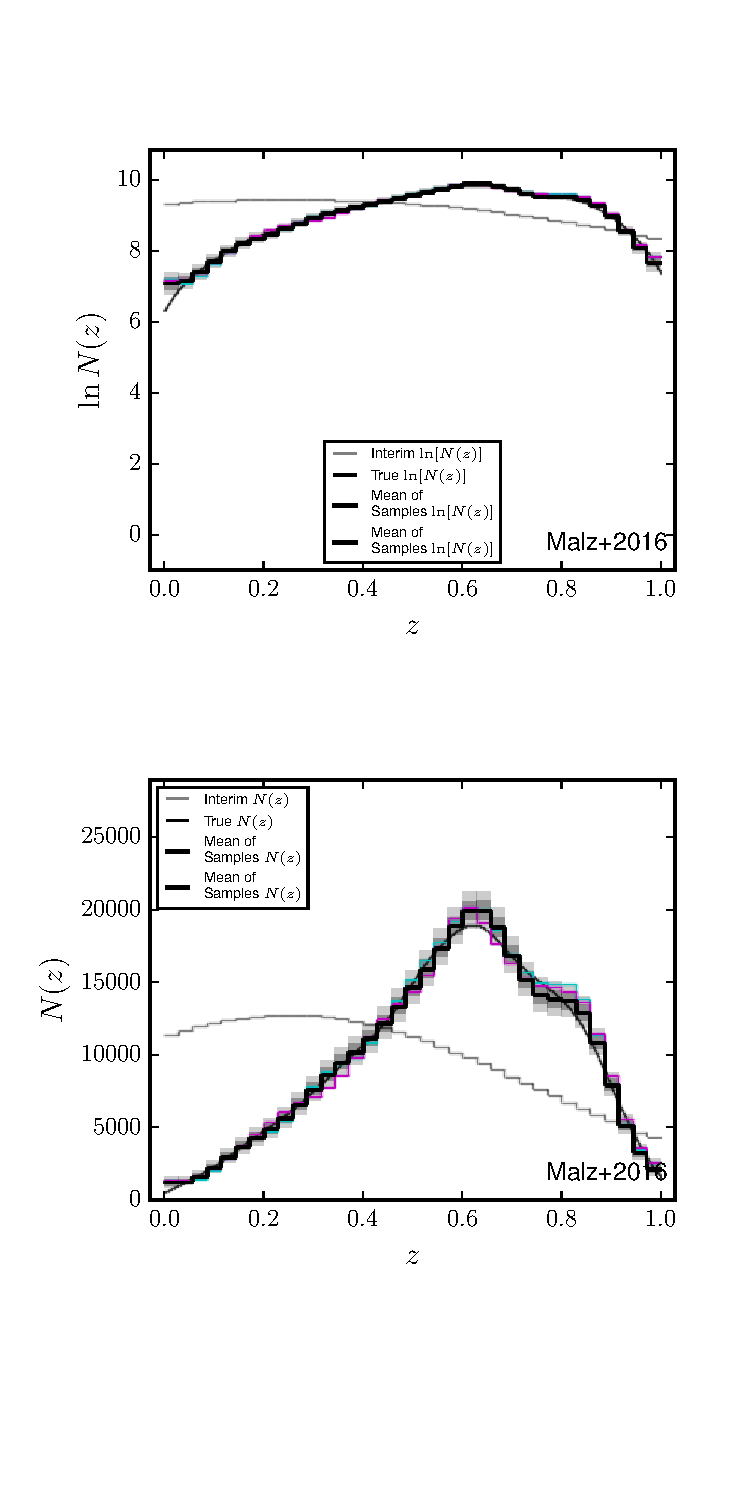
\includegraphics[width=0.5\textwidth]{figs/uint/samps.pdf}
%\caption{The mean (thick, black line) of the samples (colored lines) show no 
influence of the interim prior (gray line) and accurately replicates the 
features of the true $N(z)$ (thin, black line) everywhere that the interim 
prior supports the data.}
%\label{fig:intu-samp}
%\end{figure}

\begin{figure}
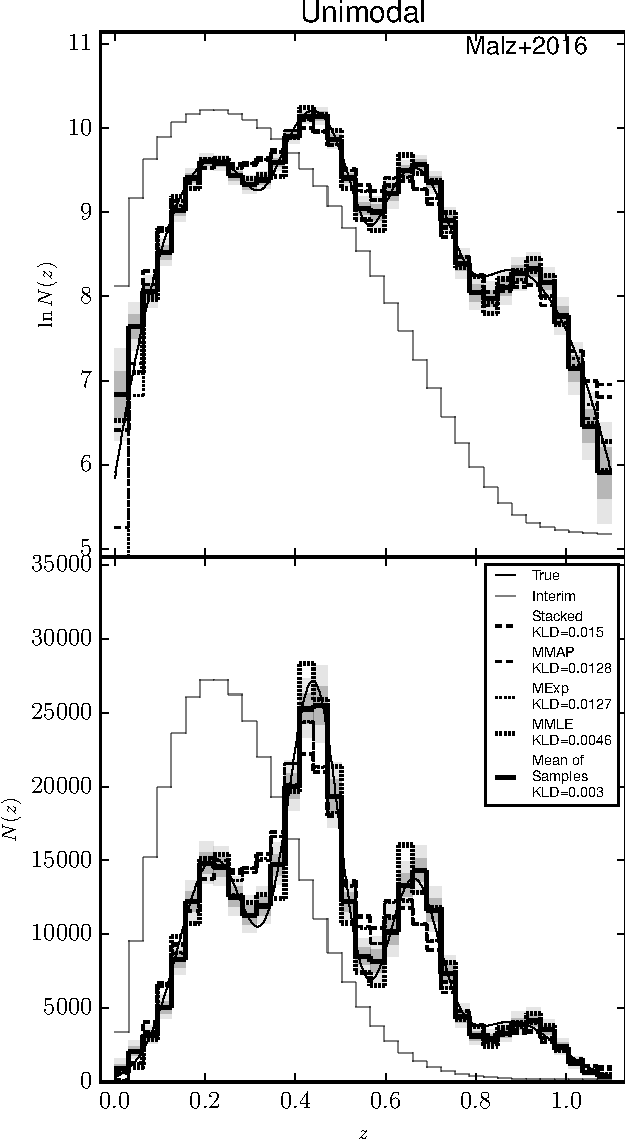
\includegraphics[width=0.5\textwidth]{figs/uint/comps.pdf}
\caption{It is clear that the interim prior (gray line) biases the result of 
stacking (dotted line), while the mean of the sampled values (thick, black 
line) is less sensitive to it and more accurately recover the true $N(z)$ 
(thin, black line).  When the interim prior does not support the full range of 
the data, the marginalized MLE (dashed line) does not converge, so the sampler 
must be preferred.}
\label{fig:intu-comp}
\end{figure}

Another potential method for selecting an interim prior with support over the 
entire redshift range expected of the photometric survey is to sum two or more 
$N(z)$ distributions obtained from reliable photometric surveys in the past.  
This is just as problematic as using a biased spectroscopically derived $N(z)$ 
as the interim prior because the sum of redshift distributions for two or more 
surveys does not reflect our beliefs about the true distribution for a single 
survey even though it provides support over the same redshift range.  To 
simulate this case, we choose an interim prior with more weight at high and low 
redshifts than for mid-range redshifts.  

Fig. \ref{fig:intb-comp} shows the comparison of the mean of the sample values 
to the true values and the result of stacking.  What is most striking is that 
stacking is very strongly affected by the choice of the interim prior, whereas 
the mean of the samples is only weakly affected by it and the marginalized MLE 
is not affected by it very much at all.  Based on these results, it can be 
concluded that when the interim prior is known to be inappropriate, the 
marginalized MLE is the best estimator of the truth.  \textbf{I'm redoing this 
test with a less exaggerated bimodal interim prior because a realistic case 
would have some overlap between the two components anyway so there is even-ish 
coverage of the entire redshift range.}

%\begin{figure}
%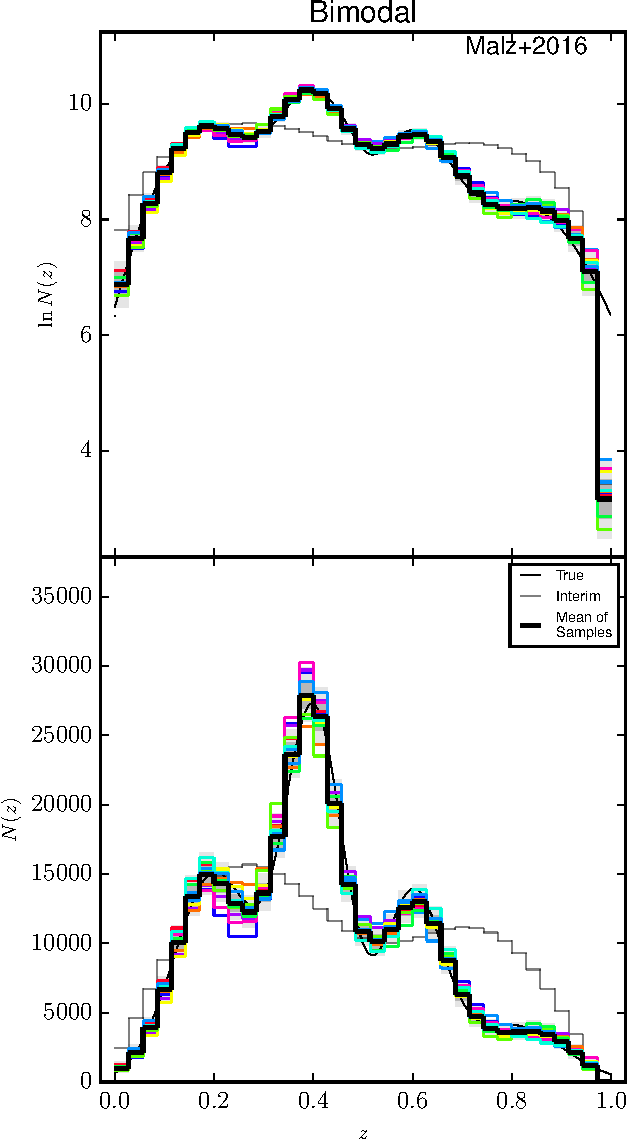
\includegraphics[width=0.5\textwidth]{figs/bint/samps.pdf}
%\caption{The mean (thick, black line) of the samples (colored lines) show some 
influence of the interim prior (gray line) but also replicate some of the 
features of the true $N(z)$ (thin, black line).}
%\label{fig:intb-samp}
%\end{figure}

\begin{figure}
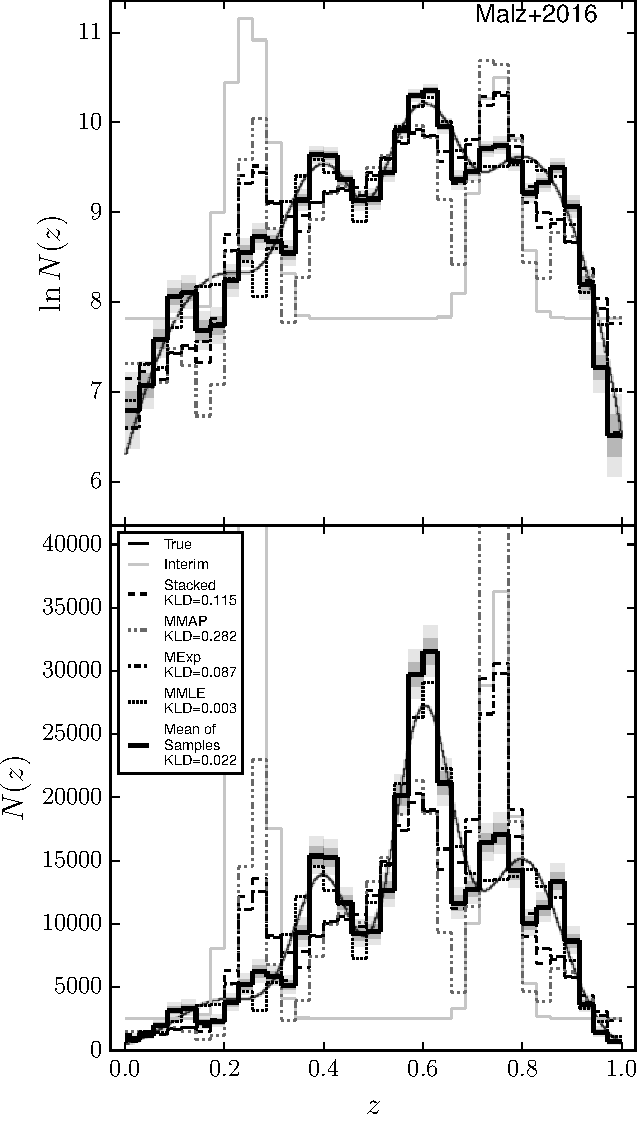
\includegraphics[width=0.5\textwidth]{figs/bint/comps.pdf}
\caption{It is clear that the result of stacking (dotted line) is strongly 
influenced by the interim prior (gray line), while the mean of the sampled 
values (thick, black line) and the marginalized MLE (dashed line) are less 
sensitive to it and more accurately recover the true $N(z)$ (thin, black line).}
\label{fig:intb-comp}
\end{figure}

\clearpage
\subsection{Data}
\label{sec:boss}

In addition to simulated tests, we also apply this method to a samples of the 
data described in Sec. \ref{sec:data}.  The interim prior is taken from 
\citet{Sheldon2012}.  In these cases the true $N(z)$ is not known, but the 
fully probabilistic method presented here may still be compared to what is 
obtained by alternative approaches.

\clearpage
\subsubsection{Unbiased Data}
\label{sec:unbiased}

A pseudo-random sampling of the full BOSS dataset is examined to approximate 
the behavior of an unbiased galaxy survey.  The results of the inference are 
shown in Fig. \ref{fig:dataparam}.

\begin{figure}
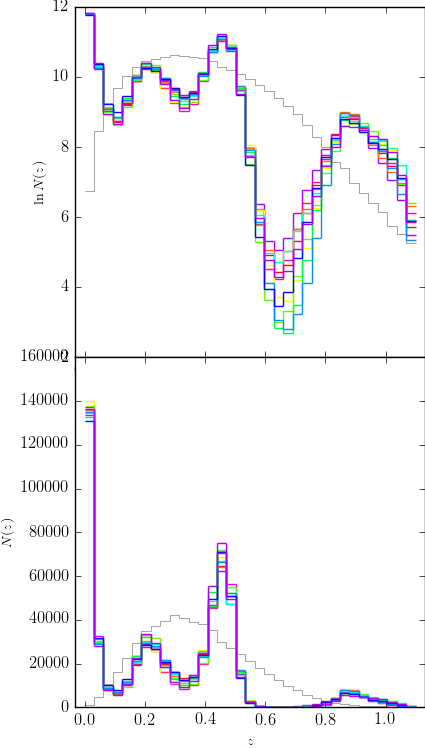
\includegraphics[width=0.5\textwidth]{figs/boss/samps.png}
\caption{Samples from the full posterior (colored lines) of the subsample 
differ substantially from the interim prior (gray).}
\label{fig:dataparam}
\end{figure}

\clearpage
\subsubsection{Biased Data}
\label{sec:biased}

A pseudo-random sampling of the full dataset with a cut in $r$-band magnitude 
is examined to approximate the behavior of a biased galaxy survey with a 
magnitude limit.  In this case, the dataset is the same as used in Sec. 
\ref{sec:boss}, excluding the dimmest half of the galaxies.  The results of the 
inference are shown in Fig. \ref{fig:biasparam}.

\begin{figure}
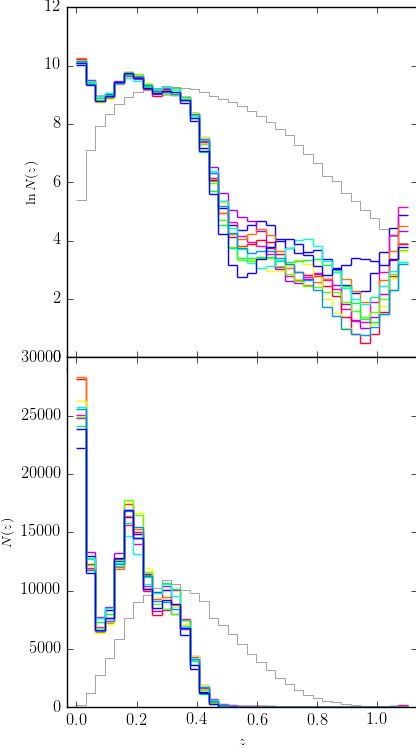
\includegraphics[width=0.5\textwidth]{figs/bias/samps.png}
\caption{Samples from the full posterior (colored lines) of the subsample 
differ substantially from the interim prior (gray) as well as the result of the 
unbiased sample.}
\label{fig:biasparam}
\end{figure}

\clearpage
\section{Conclusion}
\label{sec:con}

This study derives and demonstrates a mathematically consistent implementation 
of inference of a one-point statistic based on interim photo-z posteriors.  The 
fully Bayesian method, based in the fundamental laws of probability, begins 
with a graphical model corresponding to equations for the full posterior.  The 
technique developed in this paper is applied to the example of the redshift 
distribution function $N(z)$ with promising results on mock data; not only is 
this the only mathematically correct approach to the problem, it also recovers 
the true parameter values better than popular alternatives.  

When data suffers from imprecision, as in the case of high intrinsic scatter, 
and when data suffers from inaccuracies, as in the case of catastrophic 
outliers, the mean of sampled values is an improvement over the point estimates 
of stacking and the marginalized MLE.  In cases of perversely featured true 
redshift distributions and inappropriate but known choices of interim priors, 
the marginalized MLE is a better choice than stacking or sampling, although 
sampling still performs better than stacking.  See Tab. \ref{tab:kld} for a 
summary of the results of these comparisons.

By showing that this method is effective in recovering the true redshift 
distribution function and posterior distributions on its parameters from 
simulated interim photo-z posteriors, this work supports the production of 
interim photo-z posteriors by upcoming photometric surveys such as LSST so that 
more accurate inference of physical parameters may be accessible to the 
scientific community.  We discourage researchers from co-adding interim photo-z 
posteriors or converting them into point estimates of redshift and instead 
recommend the use of Bayesian probability to guide the usage of interim photo-z 
posteriors in science.  We emphasize to those who produce interim photo-z 
posteriors from data that it is essential to release the interim prior used in 
generating this data product in order for proper inference to be conducted by 
consumers of this information.

The method herein developed is applicable with minimal modification to other 
one-point statistics of redshift to which we will apply this method in the 
future, such as the redshift-dependent luminosity function and weak lensing 
mean distance ratio.  Future work will also include the extension of this fully 
probabilistic approach to higher-order statistics of redshift such as the 
two-point correlation function.

\textbf{What else should I be putting here?  It seems a bit terse.}

\clearpage
\textbf{I am aware something is screwed up with my references.  I'm still 
trying to find a good reference manager and have made a mess trying out a few.  
Recommendations would be appreciated.}
\bibliographystyle{apj}
\bibliography{zPDF}

\end{document}